% !TEX program = xelatex
\documentclass[11pt,a4paper]{article}
\usepackage{uav-exam}

\begin{document}

% ---------------- Титул ----------------
\begin{titlepage}
\centering
\vspace*{0cm}
{\sffamily\color{accent}\large Подготовка к экзамену\par}
\vspace{4mm}
{\sffamily\bfseries\color{skydark}\fontsize{30}{36}\selectfont Беспилотные\\[2mm] авиационные системы\par}
\vspace{4mm}
{\color{accent}\rule{0.6\linewidth}{1.2pt}\par}
\vspace{4mm}
{\sffamily\Large Конспект: законы 2026, устройство, связь, ПО\par}
\vspace{8mm}
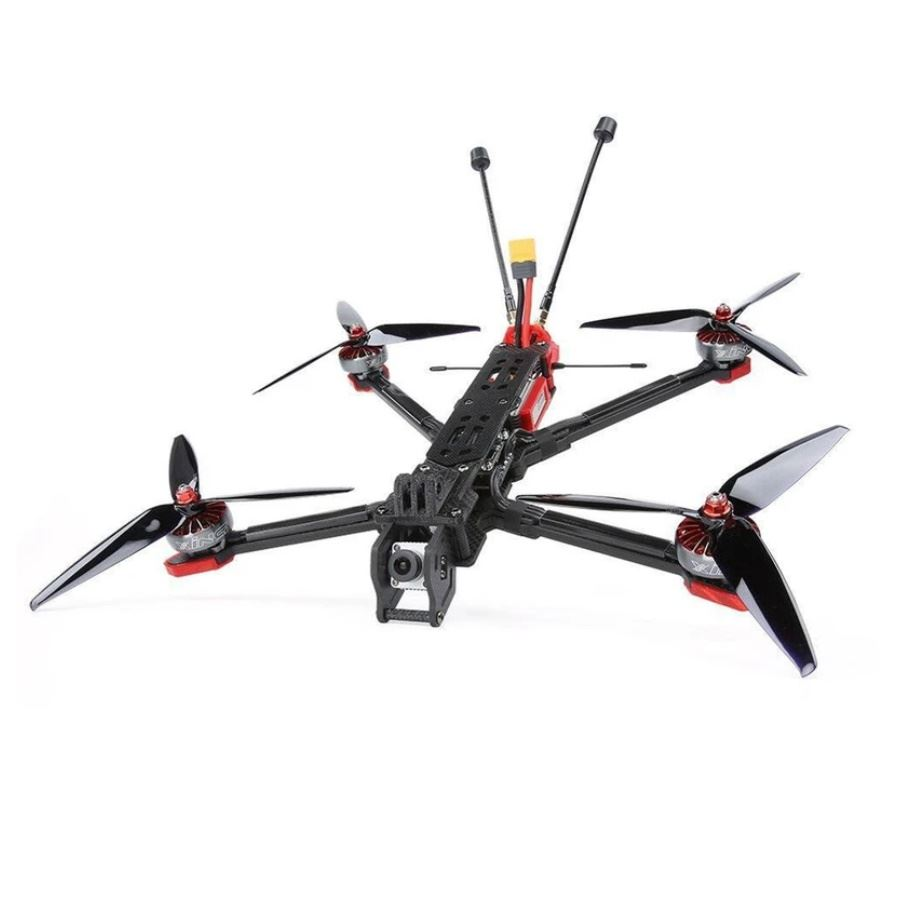
\includegraphics[width=0.62\linewidth]{img/fpv-quad.jpg}\par
\vspace{1cm}
\begin{minipage}{0.82\linewidth}\sffamily\small
\begin{enumerate}[label=\textbf{\arabic*.},itemsep=0pt]
\item Полёты в России в 2026 году, Ленинградская область и Санкт-Петербург
\item Классификация БАС
\item Из чего состоит БАС: полётный контроллер, моторы, пропеллеры, рамы, камеры, передатчики
\item Аналоговая и цифровая видеопередача
\item ПО для настройки: Betaflight, INAV, ArduPilot
\item Протоколы: UART, PWM, PPM, SBUS (и CRSF, DShot)
\item Системы управления: ELRS, FrSky, Crossfire и др.
\item Дальность связи: бюджет радиолинии, зона Френеля, горизонт
\end{enumerate}
\end{minipage}
\vfill
{\sffamily\small\color{gray} Санкт-Петербург, 2026. Фото на титуле — FPV-квадрокоптер 7" (ArduPilot Wiki)\par}
\end{titlepage}

\tableofcontents
\newpage

\section{Полёты БПЛА в России в 2026 году}

\begin{caution}[Важно помнить]
Правила меняются очень быстро — особенно региональные запреты. Ниже — состояние на сентябрь 2026 года.
Перед любым реальным полётом проверяйте актуальные документы: сайт Росавиации (\url{favt.gov.ru}),
сайт правительства своего региона и Госуслуги.
\end{caution}

\subsection{Основные термины (по Воздушному кодексу РФ)}
\begin{itemize}
\item \term{БВС} (беспилотное воздушное судно) — воздушное судно, управляемое внешним пилотом, который находится вне борта. В быту — «дрон», «БПЛА», «коптер».
\item \term{БАС} (беспилотная авиационная система) — комплекс: одно или несколько БВС + \term{станция внешнего пилота} (пульт, наземная станция) + \term{линии управления и контроля} (радиоканалы) + средства обеспечения (зарядка, транспорт и т.\,п.).
\item \term{Внешний пилот} — лицо, управляющее БВС с земли. Для БВС массой более 30~кг нужно \term{свидетельство внешнего пилота}.
\item \term{ИВП} — использование воздушного пространства. Полёт БВС на улице — это ИВП, для которого действуют \term{Федеральные правила ИВП} (Постановление Правительства РФ № 138 от 11.03.2010).
\item \term{VLOS / BVLOS} — полёт в пределах / за пределами прямой визуальной видимости пилота.
\end{itemize}

\subsection{Учёт и регистрация (федеральный уровень)}

\begin{table}[H]\centering\small
\renewcommand{\arraystretch}{1.3}
\begin{tabularx}{\linewidth}{@{}p{30mm} X X@{}}
\toprule
\textbf{Масса БВС} & \textbf{Что требуется} & \textbf{Документ} \\
\midrule
до \SI{150}{\gram} & Учёт не нужен. \emph{Но} региональные запреты и правила ИВП действуют! & ПП № 658 \\
\SIrange{0.15}{30}{\kilo\gram} & \term{Учёт} в Росавиации (через Госуслуги). Учётный номер наносится на корпус до первого полёта & ПП РФ № 658 от 25.05.2019 \\
более \SI{250}{\gram} & С \textbf{1 марта 2026} — обязательное оснащение аппаратурой удалённой идентификации / мониторинга и подключение к ГИС «ЭРА-ГЛОНАСС» (координаты, скорость, владелец — в реальном времени) & Постановление Правительства, Минтранс \\
более \SI{30}{\kilo\gram} & \term{Государственная регистрация}, сертификат лётной годности, свидетельство внешнего пилота & Воздушный кодекс РФ \\
\bottomrule
\end{tabularx}
\caption{Требования к БВС в зависимости от массы}
\end{table}

\subsection{Как законно выполнить полёт (общий порядок)}
\begin{enumerate}
\item Поставить БВС на учёт (если $m > \SI{150}{\gram}$), нанести учётный номер; с 2026 г. — подключить к «ЭРА-ГЛОНАСС» (если $m > \SI{250}{\gram}$).
\item Проверить, нет ли в месте полёта \term{запретных зон}, \term{зон ограничения полётов}, диспетчерских зон аэродромов (например, Пулково), зон вокруг режимных объектов. Проверить \textbf{региональный запрет}.
\item Над населённым пунктом — получить \term{разрешение органа местного самоуправления} (администрации).
\item Подать \term{план полёта} / заявку на установление местного режима в \term{зональный центр ЕС ОрВД} (через систему СППИ, обычно не позднее чем за сутки), в день полёта — связаться с диспетчером.
\item Выполнять полёт в светлое время суток, в пределах видимости, на безопасной высоте (типично до \SI{150}{\metre}), не над людьми и массовыми мероприятиями.
\end{enumerate}

\begin{keybox}[Полёты в помещении]
Полёт внутри здания (спортзал, аудитория, закрытая арена) \textbf{не является использованием воздушного пространства} РФ, поэтому план полёта и разрешения ЕС ОрВД не нужны. Именно поэтому учебные полёты и FPV-гонки в 2026 году проходят в залах. Нужно лишь согласие владельца помещения и соблюдение техники безопасности.
\end{keybox}

\subsection{Региональные запреты: откуда они берутся}
Указом Президента РФ № 757 от 19.10.2022 в субъектах РФ введены режимы готовности (базовый, средний, повышенный). На их основании губернаторы вправе вводить ограничения, в том числе \textbf{запрет на использование БПЛА} на территории региона. В 2025–2026 гг. такие запреты действуют в большинстве регионов европейской части России. Дополнительно при атаках БПЛА объявляется режим «\term{беспилотная опасность}»: могут ограничиваться мобильный интернет, закрываться аэропорты (режим «Ковёр»).

\subsection{Ленинградская область}
\begin{itemize}
\item С \textbf{мая 2023 года} действует \textbf{запрет на использование беспилотных воздушных судов} на всей территории области — постановление губернатора А.\,Ю.~Дрозденко.
\item Исключения — работы по специальному разрешению регионального \term{оперативного штаба} (обеспечение безопасности, инфраструктура, госзадачи). Для полётов тяжёлых БВС (свыше 30~кг) также требуется решение оперштаба.
\item Запрет действует до снятия режима базовой готовности, введённого Указом № 757.
\item В 2026 году неоднократно объявлялась «опасность БПЛА» (например, 28 июля 2026) — в это время возможны ограничения связи и транспорта.
\end{itemize}

\subsection{Санкт-Петербург}
\begin{itemize}
\item Запрет на запуск БПЛА продлён постановлением губернатора А.\,Д.~Беглова \textbf{до 31 декабря 2026 года}.
\item Тем же документом запрещена публикация фото/видео и сведений о последствиях атак БПЛА.
\item Рядом — аэропорт Пулково (диспетчерская зона), многочисленные запретные зоны над центром города.
\end{itemize}

\subsection{Ответственность}
\begin{table}[H]\centering\small
\renewcommand{\arraystretch}{1.25}
\begin{tabularx}{\linewidth}{@{}X r r r@{}}
\toprule
\textbf{Нарушение (КоАП РФ)} & \textbf{Граждане} & \textbf{Должностные} & \textbf{Юр. лица} \\
\midrule
ст. 11.4 ч.\,1 — нарушение Федеральных правил ИВП & \numrange{20}{50} тыс.\,руб. & \numrange{100}{150} тыс.\,руб. & \numrange{250}{300} тыс.\,руб. \\
ст. 11.4 — ИВП лицом, не имеющим на это права & \numrange{30}{50} тыс.\,руб. & — & — \\
Нарушение регионального запрета (режим готовности, ст. 20.6.1) & штраф & штраф & штраф \\
\bottomrule
\end{tabularx}
\caption{Штрафы за незаконные полёты (ориентировочно; суммы уточнять в действующей редакции КоАП)}
\end{table}
Кроме штрафа, дрон могут изъять, а силовые структуры вправе подавить или уничтожить БВС, нарушающий порядок ИВП. Полёт над охраняемыми объектами может повлечь уголовную ответственность.

\begin{exam}
\begin{enumerate}
\item Какие БВС подлежат учёту, а какие — государственной регистрации?
\item Что изменилось с 1 марта 2026 года?
\item Почему в Ленинградской области нельзя просто так запустить дрон? Какой документ это запрещает?
\item Нужен ли план полёта для полёта в спортзале? Почему?
\end{enumerate}
\end{exam}

\section{Классификация БАС}

Единой классификации нет — БАС делят по нескольким признакам. На экзамене обычно спрашивают: по \textbf{схеме (типу)}, по \textbf{массе}, по \textbf{дальности / радиусу}, по \textbf{способу управления} и по \textbf{назначению}.

\subsection{По аэродинамической схеме (типу летательного аппарата)}

\begin{figure}[H]\centering
\begin{subfigure}[b]{0.24\linewidth}\centering
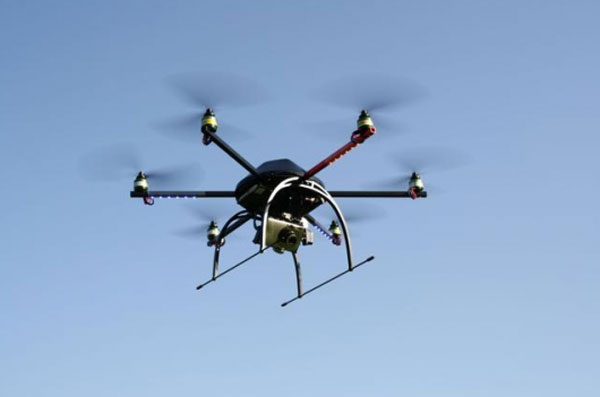
\includegraphics[width=\linewidth,height=30mm,keepaspectratio]{img/hexacopter.jpg}
\caption{Мультироторный}\end{subfigure}\hfill
\begin{subfigure}[b]{0.24\linewidth}\centering
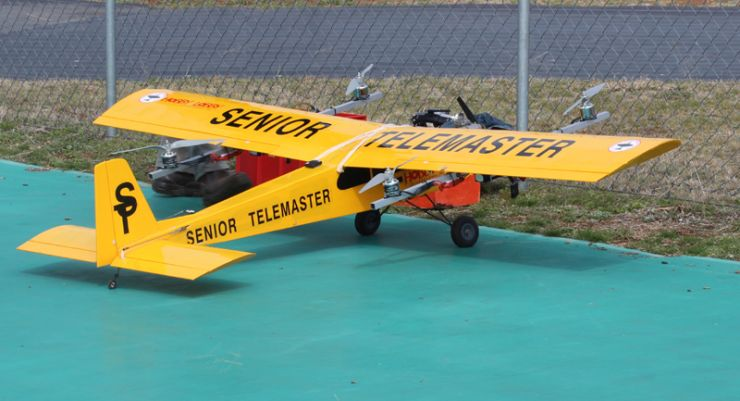
\includegraphics[width=\linewidth,height=30mm,keepaspectratio]{img/vtol.jpg}
\caption{Самолётный}\end{subfigure}\hfill
\begin{subfigure}[b]{0.24\linewidth}\centering
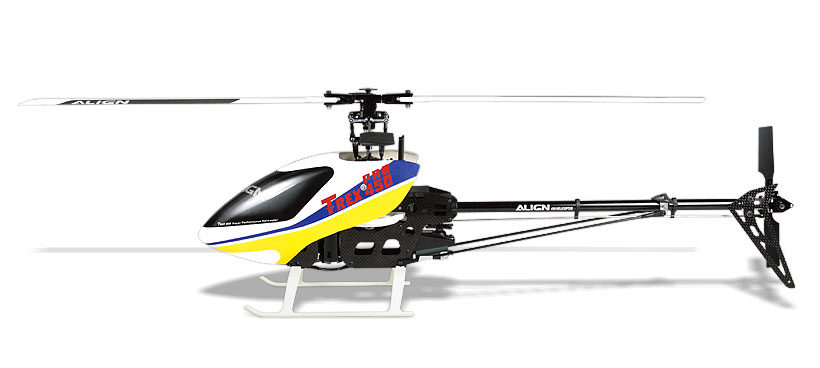
\includegraphics[width=\linewidth,height=30mm,keepaspectratio]{img/heli.jpg}
\caption{Вертолётный}\end{subfigure}\hfill
\begin{subfigure}[b]{0.24\linewidth}\centering
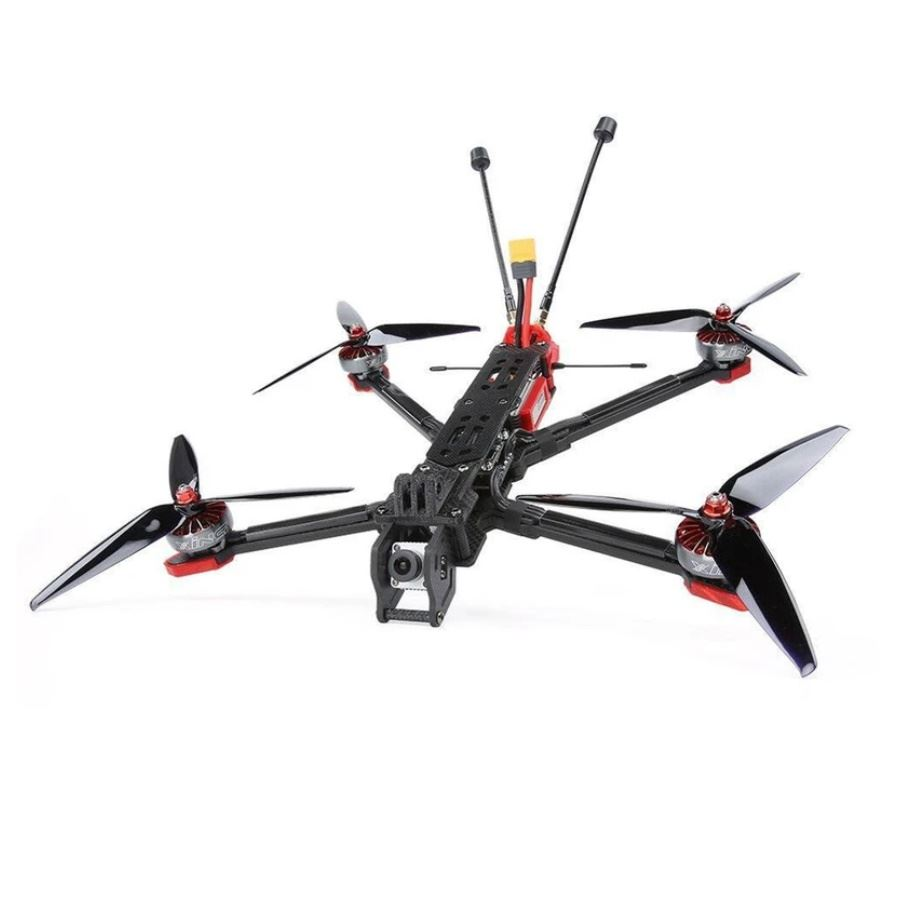
\includegraphics[width=\linewidth,height=30mm,keepaspectratio]{img/fpv-quad.jpg}
\caption{FPV-квадрокоптер}\end{subfigure}
\caption{Основные схемы БВС {\color{gray}\scriptsize(фото: ArduPilot Wiki)}}
\end{figure}

\begin{table}[H]\centering\small
\renewcommand{\arraystretch}{1.3}
\begin{tabularx}{\linewidth}{@{}>{\raggedright\arraybackslash}p{33mm} X X@{}}
\toprule
\textbf{Тип} & \textbf{Плюсы} & \textbf{Минусы} \\
\midrule
\textbf{Мультироторный} (квадро-, гекса-, октокоптер) & Вертикальный взлёт, зависание, простая механика, дешёвый & Малое время полёта (\SIrange{5}{40}{\minute}), низкий КПД \\
\textbf{Самолётного типа} (классика, «летающее крыло») & Большая дальность и время полёта (часы), высокая скорость, экономичность & Нужна площадка/катапульта для взлёта и посадки, не может зависать \\
\textbf{Вертолётного типа} & Зависание, большая грузоподъёмность, один большой ротор эффективнее & Сложная механика (автомат перекоса), сложен в обслуживании \\
\textbf{Гибридный (VTOL)} — конвертоплан, «квадроплан», tail-sitter & Взлёт как коптер, полёт как самолёт & Сложность, лишняя масса моторов в крейсерском полёте \\
\textbf{Аэростатный / привязной} & Очень долгое нахождение в воздухе & Зависимость от ветра, большие размеры \\
\bottomrule
\end{tabularx}
\caption{Сравнение схем}
\end{table}

\subsection{По массе}
\begin{itemize}
\item \textbf{Правовая (РФ)}: до \SI{0.15}{\kilo\gram} — без учёта; \SIrange{0.15}{30}{\kilo\gram} — учёт; более \SI{30}{\kilo\gram} — государственная регистрация (см. раздел 1).
\item \textbf{Техническая (распространённая)}: \emph{нано/микро} — до \SI{0.25}{\kilo\gram} (tiny whoop, DJI Mini); \emph{мини} — до \SIrange{5}{7}{\kilo\gram}; \emph{лёгкие} — до \SI{30}{\kilo\gram}; \emph{средние} — до \SI{150}{\kilo\gram}; \emph{тяжёлые} — более \SI{150}{\kilo\gram}.
\end{itemize}

\subsection{По дальности (радиусу действия) и высоте}
\begin{table}[H]\centering\small
\begin{tabularx}{\linewidth}{@{}l >{\raggedright\arraybackslash}X >{\raggedright\arraybackslash}X@{}}
\toprule
\textbf{Класс} & \textbf{Радиус} & \textbf{Пример} \\
\midrule
Ближнего действия (Close Range) & до \SIrange{10}{30}{\kilo\metre} & FPV-дроны, DJI Mavic, «Геоскан 201» \\
Малой дальности (Short Range) & \SIrange{30}{70}{\kilo\metre} & «Орлан-10»\\
Средней дальности (Medium Range) & \SIrange{70}{200}{\kilo\metre} & — \\
MALE (Medium Altitude Long Endurance) & сотни км, высота до \SI{9}{\kilo\metre}, 24+ ч & «Орион», MQ-1 \\
HALE (High Altitude Long Endurance) & тысячи км, высота до \SI{20}{\kilo\metre} & RQ-4 Global Hawk \\
\bottomrule
\end{tabularx}
\caption{Классификация по дальности (по UVS International)}
\end{table}

\subsection{По способу управления}
\begin{itemize}
\item \term{Ручное (дистанционно пилотируемое)} — пилот управляет в реальном времени: по прямой видимости (LOS) или по видео (\term{FPV}, First Person View — «вид от первого лица»).
\item \term{Автоматическое} — полёт по заранее заданной программе (миссии по точкам GPS), пилот контролирует и может вмешаться.
\item \term{Автономное} — БВС сам принимает решения (обход препятствий, распознавание целей, навигация без GNSS).
\end{itemize}

\subsection{По назначению}
Гражданские (аэрофотосъёмка, картография, мониторинг ЛЭП и трубопроводов, сельское хозяйство — опрыскиватели, доставка, МЧС, спорт/FPV-гонки, кино), государственные (полиция, пограничники), военные (разведка, корректировка, ударные). \par
Для FPV-дронов отдельно используют \textbf{классификацию по размеру пропеллера}: \emph{whoop} 1–2" (\SIrange{65}{85}{\milli\metre}), \emph{cinewhoop} 2,5–3,5" (с защитой пропеллеров), \emph{freestyle/racing} 5", \emph{long range} 7", \emph{heavy} 8–10"+.

\begin{exam}
\begin{enumerate}
\item Назовите преимущества и недостатки мультироторной и самолётной схем.
\item Что такое VTOL и зачем он нужен?
\item Чем автоматическое управление отличается от автономного?
\end{enumerate}
\end{exam}

\section{Из чего состоит БАС}

\subsection{Общая структура}

\begin{figure}[H]\centering
\begin{tikzpicture}[font=\sffamily\small,x=0.91cm,y=1cm,
  wave/.style={decorate,decoration={snake,amplitude=.9mm,segment length=4mm,post length=2mm}}]
% Наземная часть
\node[blk,fill=blk3,minimum width=31mm] (tx)  at (0,3.2)  {Пульт (аппаратура)\\+ TX-модуль};
\node[blk,fill=blk3,minimum width=31mm] (gog) at (0,1.2)  {Очки / монитор\\+ видеоприёмник};
\node[blk,fill=blk3,minimum width=31mm] (gcs) at (0,-2.4) {Наземная станция\\(ноутбук, GCS)};
\node[draw,dashed,rounded corners,fit=(tx)(gog)(gcs),inner sep=3mm,label={[font=\sffamily\bfseries]above:Станция внешнего пилота}] {};
% Борт
\node[blk,fill=blk2,minimum width=22mm] (rx)  at (6.6,3.2)  {Приёмник RC};
\node[blk,fill=blk2,minimum width=22mm] (gps) at (9.6,3.2)  {GPS + компас};
\node[blk,fill=gray!15] (pl) at (13.4,3.2) {Полезная нагрузка\\(гимбал, камера)};
\node[blk,fill=blk1,minimum width=24mm] (fc)  at (8.1,1.2)  {\textbf{Полётный}\\\textbf{контроллер}\\(IMU, баро, МК)};
\node[blk,fill=blk4] (esc) at (11.6,1.2) {ESC\\(регуляторы)};
\node[blk,fill=blk4] (mot) at (14.4,1.2) {Моторы\\+ пропеллеры};
\node[blk,fill=blk2,minimum width=22mm] (vtx) at (6.3,-0.9) {VTX\\(видеопередатчик)};
\node[blk,fill=blk2,minimum width=20mm] (cam) at (10.0,-0.9) {FPV-камера};
\node[blk,fill=blk5] (bat) at (12.9,-0.9) {АКБ\\LiPo / Li-Ion};
\node[draw,dashed,rounded corners,fit=(rx)(pl)(mot)(vtx)(bat),inner sep=3mm,label={[font=\sffamily\bfseries]above:Беспилотное воздушное судно}] {};
% Провода на борту
\draw[arr] (rx) -- (fc); \draw[arr] (gps) -- (fc);
\draw[arr] (fc) -- node[above,font=\sffamily\scriptsize]{DShot} (esc); \draw[arr] (esc) -- (mot);
\draw[arr] (cam) -- (vtx); \draw[arr] (fc) -- node[left,font=\sffamily\scriptsize]{OSD} (vtx);
\draw[arr] (bat) -- (esc);
% Радиоканалы
\draw[arr,accent,wave] (tx.east) -- node[below=1.5mm,font=\sffamily\scriptsize]{RC: 2,4\,ГГц / 868\,МГц} (rx.west);
\draw[arr,okgreen,wave] (vtx.west) -- node[below=1.5mm,sloped,font=\sffamily\scriptsize]{видео 5,8\,ГГц} (gog.east);
\draw[warn,thick,wave] (gcs.east) -- node[below=1mm,font=\sffamily\scriptsize]{телеметрия MAVLink} (8.1,-2.4);
\draw[arr,warn] (8.1,-2.4) -- (fc.south);
\end{tikzpicture}
\caption{Состав БАС: бортовая часть, станция внешнего пилота и радиолинии}
\end{figure}

\subsection{Полётный контроллер (ПК, FC — Flight Controller)}
\term{Полётный контроллер} — «мозг» дрона. Несколько тысяч раз в секунду он читает датчики, сравнивает фактическое положение с командой пилота и через \term{ПИД-регулятор} вычисляет, с какой тягой должен крутиться каждый мотор.

\begin{itemize}
\item \term{Микроконтроллер}: STM32F405/F411 (F4), F722/F745 (F7), H743 (H7), AT32F435. Чем «старше» серия, тем больше частота, память и UART-портов. F411 — только 2–3 UART, H7 — до 8.
\item \term{IMU} (инерциальный модуль): гироскоп + акселерометр — MPU6000, ICM-42688-P, BMI270. Гироскоп — главный датчик стабилизации.
\item \term{Барометр} (BMP280, DPS310) — высота; \term{магнитометр} (компас) — курс; \term{OSD-чип} (AT7456E) — наложение телеметрии на аналоговое видео; \term{Blackbox} — флеш-память для логов.
\item \term{Порты}: UART (приёмник, GPS, VTX, телеметрия), I2C (компас, дисплей), SPI (IMU), выходы на моторы/сервы, USB для настройки.
\item \term{Монтажные размеры} (расстояние между отверстиями): 30,5×30,5~мм, 20×20~мм, 25,5×25,5~мм (whoop), 16×16~мм.
\item \term{Стек} — ПК + плата ESC «бутербродом»; \term{AIO} (All-In-One) — ПК, ESC, иногда приёмник и VTX на одной плате (для микро-дронов).
\end{itemize}

\begin{figure}[H]\centering
\begin{minipage}[b]{0.30\linewidth}\centering
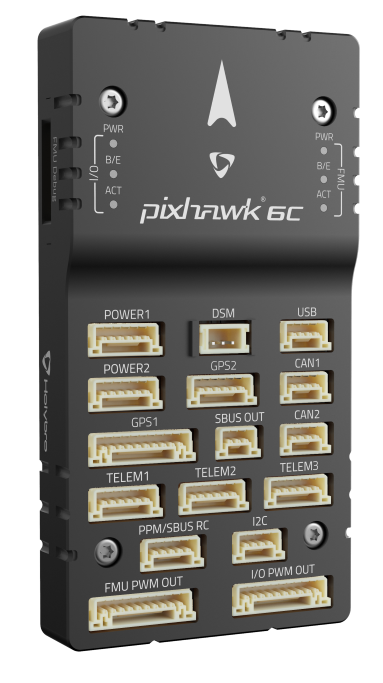
\includegraphics[width=\linewidth]{img/pixhawk6c.png}\\[-1mm]
{\small\textbf{Pixhawk 6C} — автопилот для ArduPilot/PX4}
\end{minipage}\hfill
\begin{minipage}[b]{0.30\linewidth}\centering
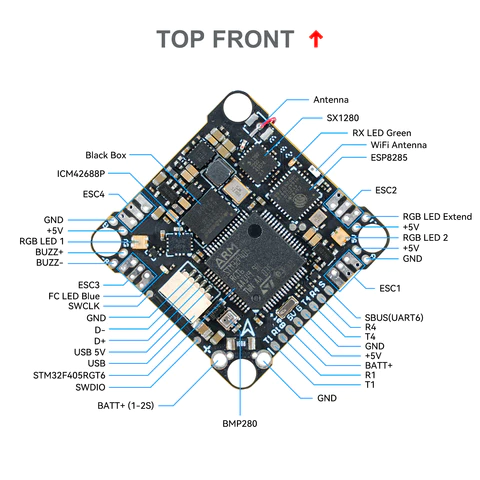
\includegraphics[width=\linewidth]{img/f405-top.png}\\[-1mm]
{\small\textbf{F405 AIO} — FPV-контроллер для Betaflight/INAV}
\end{minipage}\hfill
\begin{minipage}[b]{0.35\linewidth}\centering
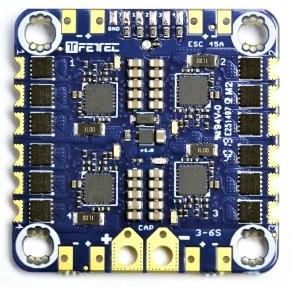
\includegraphics[width=\linewidth]{img/esc4in1.jpg}\\[-1mm]
{\small\textbf{ESC 4-в-1} — четыре регулятора на одной плате}
\end{minipage}
\caption{Полётные контроллеры и регулятор оборотов {\color{gray}\scriptsize(фото: ArduPilot Wiki)}}
\end{figure}

\photo{0.85\linewidth}{f405-wiring.png}{Типовая схема подключения FPV-контроллера: камера, цифровой VTX, приёмник ELRS/TBS, GPS, пищалка, светодиоды}{ArduPilot Wiki}

\subsection{Регуляторы оборотов (ESC)}
\term{ESC} (Electronic Speed Controller) превращает постоянное напряжение батареи в трёхфазное для бесколлекторного мотора, переключая MOSFET-ключи. Характеристики: \textbf{ток} (например, 45\,А длительно), \textbf{напряжение} (3–6S), прошивка (\textbf{BLHeli\_S}, \textbf{Bluejay}, \textbf{BLHeli\_32}, \textbf{AM32}) и протокол связи с ПК (PWM, OneShot, MultiShot, \textbf{DShot} — см. раздел 6). \term{Двунаправленный DShot} передаёт обороты мотора обратно в ПК для RPM-фильтра.

\subsection{Моторы}
\begin{table}[H]\centering\small
\renewcommand{\arraystretch}{1.3}
\begin{tabularx}{\linewidth}{@{}p{34mm} X@{}}
\toprule
\textbf{Коллекторные} (brushed, 6×15, 8×20~мм) & Щётки + коллектор. Дёшевы, управляются одним транзистором (ШИМ). Износ щёток, малый ресурс. Только микро-дроны и игрушки. \\
\textbf{Бесколлекторные} (BLDC, brushless) & Нет щёток, коммутацию делает ESC. Высокий КПД и ресурс, большая мощность. Стандарт для всех дронов. \\
\quad — \textbf{outrunner} & Вращается внешний колокол с магнитами, статор с обмотками неподвижен внутри. Большой момент — прямой привод пропеллера. Используется на дронах. \\
\quad — \textbf{inrunner} & Вращается внутренний ротор. Высокие обороты, малый момент — для импеллеров, машинок, с редуктором. \\
\bottomrule
\end{tabularx}
\caption{Виды моторов}
\end{table}

\begin{figure}[H]\centering
\begin{minipage}[c]{0.3\linewidth}\centering
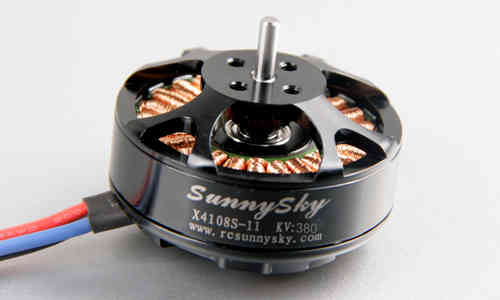
\includegraphics[width=\linewidth]{img/motor-sunny.jpg}\\
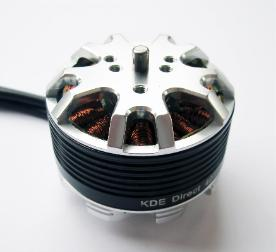
\includegraphics[width=0.8\linewidth]{img/motor-kde.jpg}\\
{\scriptsize\color{gray}(фото: ArduPilot Wiki)}
\end{minipage}\hfill
\begin{minipage}[c]{0.66\linewidth}
\begin{keybox}[Как читать маркировку мотора: \texttt{2207 1950KV}]
\begin{itemize}[leftmargin=4mm]
\item \textbf{22} — диаметр статора, мм; \textbf{07} — высота статора, мм. Больше статор — больше момент и масса.
\item \textbf{KV} — число оборотов в минуту на 1 вольт без нагрузки.\\
$n \approx KV \cdot U$: $1950 \cdot 16{,}8~\text{В} \approx 32\,760$~об/мин.
\item \textbf{Высокий KV} — маленькие лёгкие пропеллеры, низкое напряжение (гонки, 4S).\\
\textbf{Низкий KV} — большие пропеллеры, высокое напряжение (6S, дальнолёты, грузовые).
\item Типично: 5" на 6S — 1700–1950KV; 7" на 6S — 1300KV; 15" на 6–12S — 100–400KV.
\end{itemize}
\end{keybox}
\end{minipage}
\caption{Бесколлекторные моторы-outrunner}
\end{figure}

\subsection{Пропеллеры}
\begin{itemize}
\item \term{Маркировка}: диаметр × шаг (в дюймах) × число лопастей. \code{5146} или \code{5.1x4.6x3} — диаметр 5,1", шаг 4,6", 3 лопасти. \textbf{Шаг} — расстояние, на которое винт «ввинтился» бы в воздух за один оборот.
\item \term{Больше диаметр} — выше КПД и тяга, но медленнее отклик. \term{Больше шаг} — выше скорость, но больший ток. \term{Больше лопастей} — больше тяги при том же диаметре, но ниже КПД.
\item \term{Направление}: CW (по часовой) и CCW (против часовой). Соседние моторы вращаются в разные стороны, чтобы компенсировать реактивный момент (благодаря этому возможен поворот по рыскания). «Props in» / «props out» — направление вращения относительно рамы.
\item \term{Материалы}: пластик (PC), нейлон со стекловолокном — для FPV (гнутся, не ломают моторы); \term{карбон} — жёсткие, эффективные, для больших коптеров; \term{складные} — для самолётов и мультикоптеров, которые переносят в рюкзаке.
\item \term{Крепление}: на вал с гайкой (M5), T-mount (болты), для микро — на вал с натягом.
\end{itemize}

\begin{figure}[H]\centering
\begin{minipage}[b]{0.32\linewidth}\centering
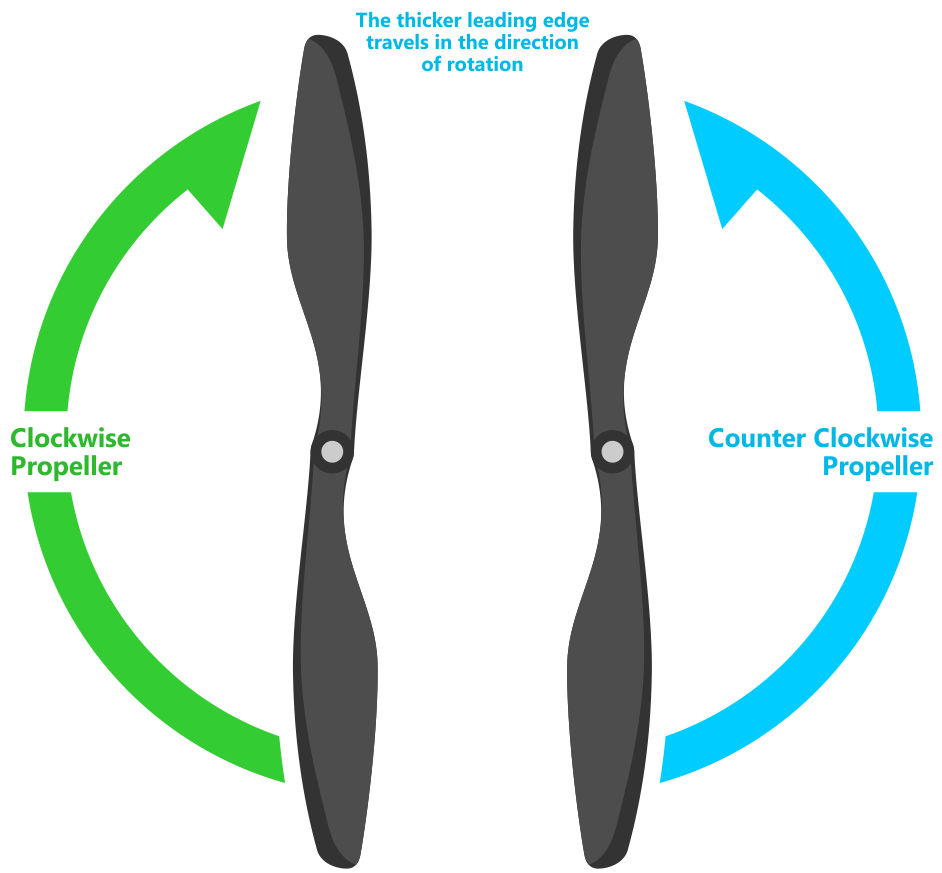
\includegraphics[width=\linewidth]{img/prop-dir.png}\\
{\small Направление вращения CW/CCW}
\end{minipage}\hfill
\begin{minipage}[b]{0.32\linewidth}\centering
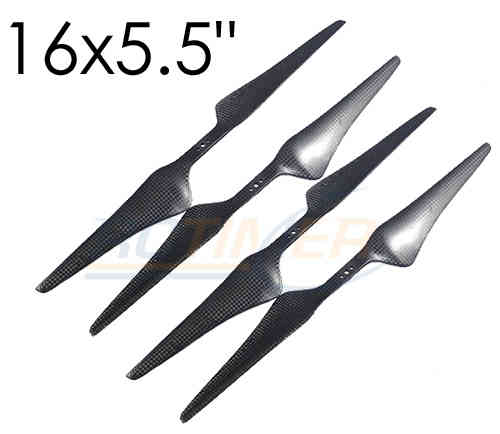
\includegraphics[width=\linewidth]{img/props.jpg}\\
{\small Пластиковые пропеллеры}
\end{minipage}\hfill
\begin{minipage}[b]{0.32\linewidth}\centering
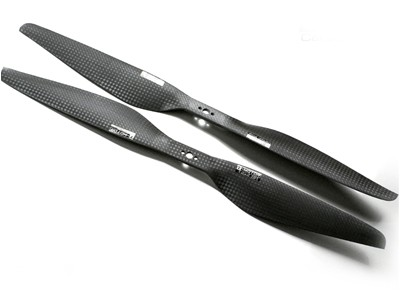
\includegraphics[width=\linewidth]{img/tmotor-props.jpg}\\
{\small Карбоновые пропеллеры для тяжёлых коптеров}
\end{minipage}
\caption{Виды пропеллеров {\color{gray}\scriptsize(фото: ArduPilot Wiki)}}
\end{figure}

\subsection{Типы рам}
\term{Рама} — несущая конструкция, к которой крепится вся электроника. Материал — \textbf{карбон} (углепластик: лёгкий и прочный), реже пластик (whoop), алюминий, стеклотекстолит. Размер задаётся \term{диагональю} (wheelbase) — расстоянием между осями противоположных моторов: 5" $\approx$ \SIrange{210}{230}{\milli\metre}, 7" $\approx$ \SI{300}{\milli\metre}.

\begin{figure}[H]\centering
\foreach \f/\n in {quadx/Quad X,quadplus/Quad +,quadh/Quad H,tri/Трикоптер}{%
\begin{minipage}[b]{0.22\linewidth}\centering
\includegraphics[height=32mm]{img/\f.png}
\end{minipage}\hfill}
\\[3mm]
\foreach \f/\n in {hexax/Hexa X,y6/Y6,octox/Octo X,x8/X8}{%
\begin{minipage}[b]{0.22\linewidth}\centering
\includegraphics[height=32mm]{img/\f.png}
\end{minipage}\hfill}
\caption{Схемы рам и порядок моторов (номер — порядок выхода ПК, CW/CCW — направление вращения). Y6 и X8 — \emph{коаксиальные}: два мотора на одном луче, один над другим {\color{gray}\scriptsize(рисунки: ArduPilot Wiki)}}
\end{figure}

\begin{table}[H]\centering\small
\renewcommand{\arraystretch}{1.25}
\begin{tabularx}{\linewidth}{@{}p{38mm} X@{}}
\toprule
\textbf{Рама} & \textbf{Особенности} \\
\midrule
\textbf{True X} & Моторы на одинаковом расстоянии по всем осям — одинаковое поведение по крену и тангажу. Фристайл. \\
\textbf{Stretched X, Squashed X} & Растянута вдоль / поперёк — оптимизация под гонки или стабильность. \\
\textbf{Deadcat} & Передние лучи разведены, чтобы пропеллеры не попадали в кадр камеры. \\
\textbf{H} & Лучи крепятся к длинной центральной балке — много места для электроники. \\
\textbf{Plus (+)} & Один мотор впереди. Сегодня используется редко. \\
\textbf{Tri} & 3 мотора + сервопривод на хвосте для управления рысканием. \\
\textbf{Hexa, Octo} & 6 и 8 моторов — грузоподъёмность и \textbf{резервирование}: при отказе одного мотора можно сесть. \\
\textbf{Коаксиальные (Y6, X8)} & Компактнее при той же тяге, но нижний винт работает в потоке верхнего (потеря КПД \SIrange{15}{25}{\percent}). \\
\bottomrule
\end{tabularx}
\caption{Особенности рам}
\end{table}

\subsection{Аккумуляторы}
\begin{itemize}
\item \term{LiPo} — литий-полимер. Ячейка: \SI{3.7}{\volt} номинал, \SI{4.2}{\volt} полный заряд, не разряжать ниже \SIrange{3.3}{3.5}{\volt}. \textbf{\emph{n}S} — число последовательных ячеек: 4S = \SI{14.8}{\volt}, 6S = \SI{22.2}{\volt}. \textbf{\emph{m}P} — параллельные.
\item \term{C-рейтинг} — допустимый ток разряда: $I_\text{max} = C \cdot Q$. Пример: \SI{1300}{\milli\ampere\hour}, 100C $\Rightarrow$ \SI{130}{\ampere}.
\item \term{LiHV} — до \SI{4.35}{\volt}/ячейка; \term{Li-Ion} (18650, 21700) — больше ёмкость на массу, меньше ток: для дальнолётов и самолётов.
\item Хранение — при \SI{3.8}{\volt}/ячейка, заряд — балансирным зарядным устройством, в негорючем мешке.
\end{itemize}

\subsection{Камеры}
\begin{table}[H]\centering\small
\renewcommand{\arraystretch}{1.25}
\begin{tabularx}{\linewidth}{@{}p{36mm} X@{}}
\toprule
\textbf{FPV-камера аналоговая} & CMOS-матрица, выход — композитный видеосигнал PAL/NTSC, 600–1200 ТВЛ. Минимальная задержка. Размеры корпуса: nano 14~мм, micro 19~мм, mini 22~мм, full 28~мм. Параметры: фокусное расстояние (1,8–2,1~мм — широкий угол), WDR, чувствительность в люксах. Примеры: RunCam Phoenix, Caddx Ratel, Foxeer Razer. \\
\textbf{FPV-камера цифровая} & Идёт в паре со своим цифровым передатчиком: DJI O3/O4, Walksnail Avatar, HDZero, OpenIPC. 720p–4K. \\
\textbf{Экшн-камера / «голая» GoPro} & Запись качественного видео (4K, стабилизация), отдельно от FPV-камеры. \\
\textbf{Камера на подвесе (гимбале)} & Аэрофотосъёмка: 2- или 3-осевой стабилизатор с бесколлекторными моторами. \\
\textbf{Тепловизор} & ИК-диапазон 8–14~мкм: поиск людей, животных, утечек тепла, ночные полёты. \\
\textbf{Ночная / мультиспектральная} & Съёмка при низкой освещённости; мультиспектр — оценка состояния посевов (NDVI). \\
\bottomrule
\end{tabularx}
\caption{Виды камер}
\end{table}

\begin{figure}[H]\centering
\begin{minipage}[b]{0.30\linewidth}\centering
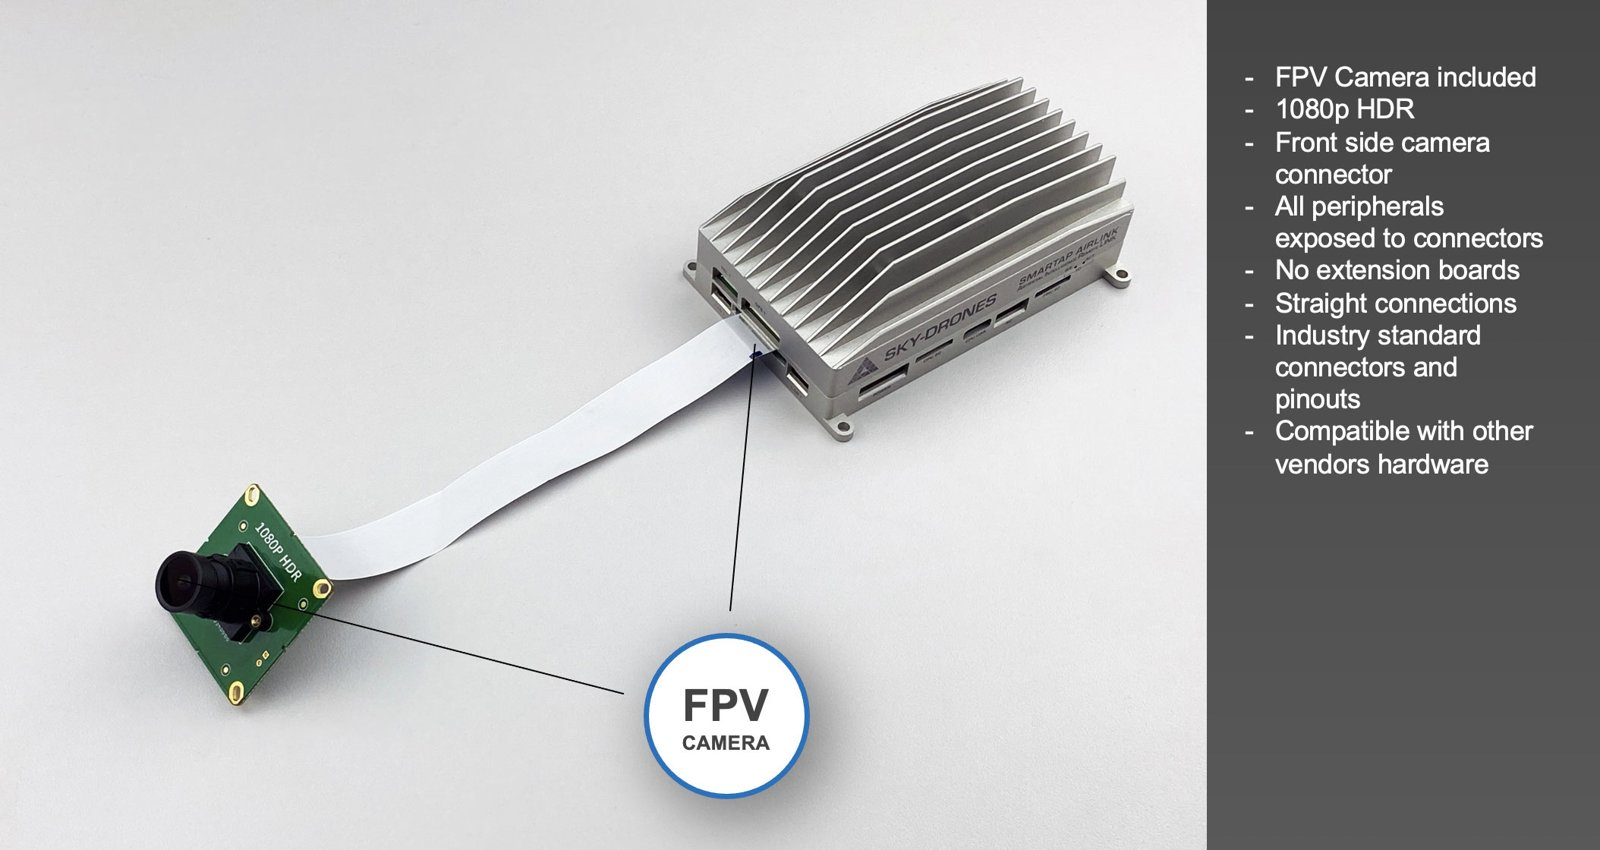
\includegraphics[width=\linewidth]{img/fpvcam.jpg}\\{\small Модуль FPV-камеры}
\end{minipage}\hfill
\begin{minipage}[b]{0.38\linewidth}\centering
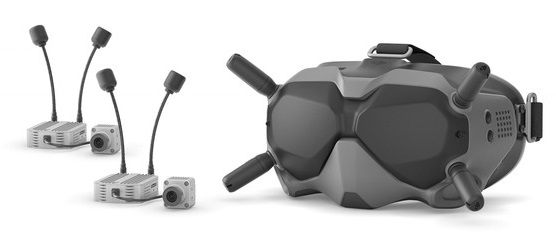
\includegraphics[width=\linewidth]{img/djifpv.jpg}\\{\small Цифровая система DJI: камеры, модули и очки}
\end{minipage}\hfill
\begin{minipage}[b]{0.28\linewidth}\centering
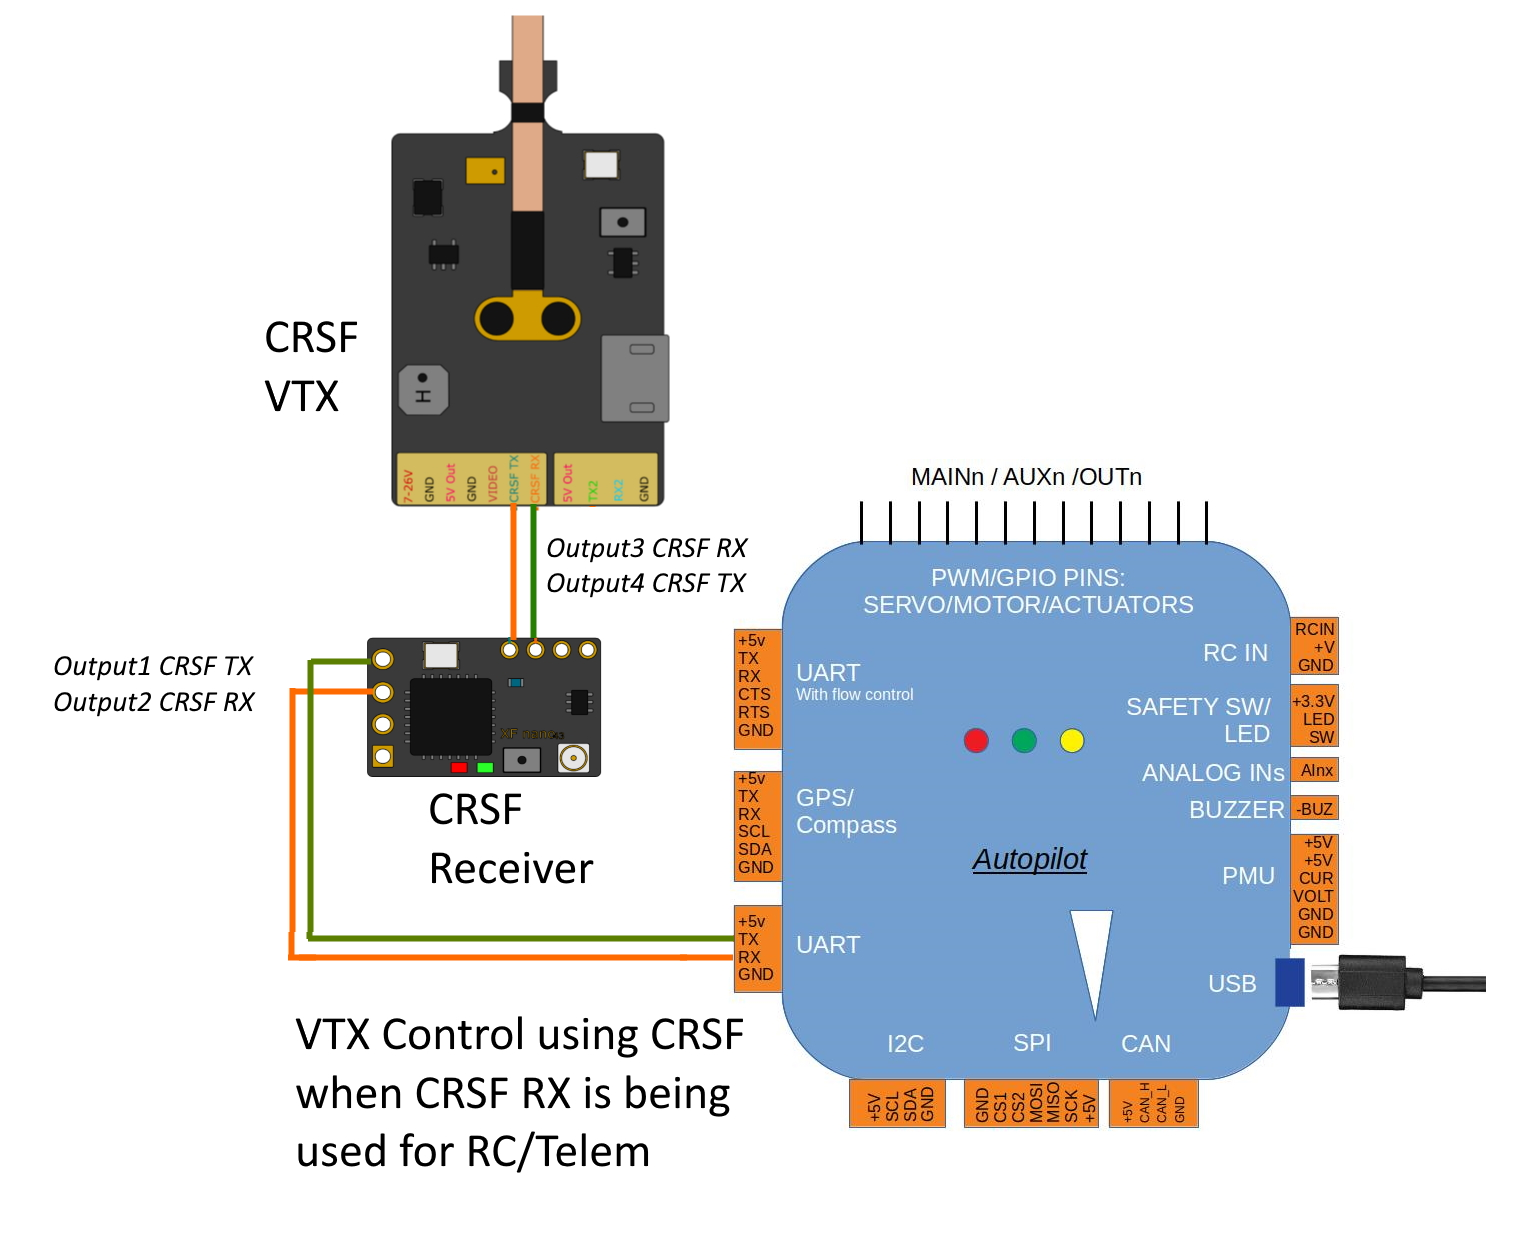
\includegraphics[width=\linewidth]{img/vtx.jpg}\\{\small Подключение VTX с управлением по UART}
\end{minipage}
\caption{Камеры и видеопередатчики {\color{gray}\scriptsize(фото: ArduPilot Wiki)}}
\end{figure}

\subsection{Передатчики и приёмники}
На борту обычно \textbf{три} радиосистемы:
\begin{enumerate}
\item \term{Приёмник управления (RX)} — получает команды от пульта (ELRS, TBS Crossfire, FrSky\ldots). Подключается к ПК по UART (CRSF, SBUS) — см. разделы 6–7.
\item \term{Видеопередатчик (VTX)} — передаёт видео с камеры в очки. Аналоговые: 5,8~ГГц (также 1,2–1,3 и 3,3~ГГц), мощность 25–2000~мВт, 40–48 каналов в диапазонах A, B, E, F (Fatshark), R (Raceband). Управляется от ПК по \textbf{SmartAudio}, \textbf{Tramp} или \textbf{MSP}.
\item \term{Модем телеметрии} — двусторонний канал с наземной станцией (MAVLink): SiK-радио 433/\allowbreak 868/\allowbreak 915~МГц, RFD900, Wi-Fi, LTE-модемы. Часто телеметрия идёт через RC-линк (ELRS, Crossfire).
\end{enumerate}

\subsection{Антенны}
\begin{itemize}
\item \term{Всенаправленные}: \textbf{диполь} (линейная поляризация), \textbf{«клевер»} (cloverleaf), \textbf{«пагода»}, \textbf{Lollipop} — круговая поляризация (RHCP/LHCP). Круговая поляризация уменьшает замирания от отражённого сигнала. \textbf{Поляризация на передатчике и приёмнике должна совпадать!}
\item \term{Направленные}: \textbf{патч}, \textbf{спиральная (helical)}, \textbf{Yagi}, \textbf{moxon} — больше усиление (дальность), но узкий луч, нужно направлять на дрон (часто — трекер).
\item \term{Разъёмы}: SMA, RP-SMA, MMCX, u.FL (IPEX). \textbf{Никогда не включайте передатчик без антенны} — выгорит выходной усилитель.
\end{itemize}

\begin{figure}[H]\centering
\begin{minipage}[b]{0.3\linewidth}\centering
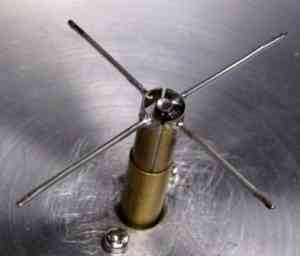
\includegraphics[width=\linewidth]{img/crossantenna.jpg}\\{\small Всенаправленная антенна с круговой поляризацией}
\end{minipage}\hspace{1cm}
\begin{minipage}[b]{0.3\linewidth}\centering
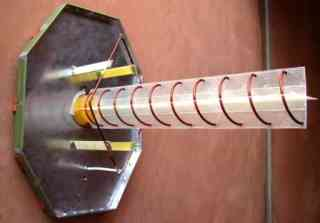
\includegraphics[width=\linewidth]{img/helical.jpg}\\{\small Направленная спиральная (helical) антенна}
\end{minipage}
\caption{Антенны {\color{gray}\scriptsize(фото: ArduPilot Wiki)}}
\end{figure}

\subsection{Прочие компоненты}
\term{GPS/ГЛОНАСС-модуль} с компасом (M8N, M10, BN-880) — позиционирование, возврат домой. \term{PDB / BEC} — распределение питания и стабилизированные 5/9/12~В. \term{Датчик тока} — расход ёмкости. \term{Дальномер, оптический поток} — удержание позиции без GPS. \term{Пищалка} (buzzer) — поиск упавшего дрона. \term{Светодиоды}, \term{парашют}, \term{сбросник} груза.

\begin{exam}
\begin{enumerate}
\item Какие датчики есть на полётном контроллере и зачем каждый?
\item Расшифруйте маркировку мотора 2306 2450KV и пропеллера 5143.
\item Зачем соседние моторы вращаются в разные стороны?
\item Чем отличаются рамы True X, Deadcat и H? В чём плюс гексакоптера перед квадрокоптером?
\item Какой ток может отдать АКБ 6S 1500~мА·ч 120C? Какое у неё напряжение при полном заряде?
\end{enumerate}
\end{exam}

\section{Аналоговая и цифровая видеопередача}

\subsection{Как работает аналоговая система}
\begin{figure}[H]\centering
\begin{tikzpicture}[node distance=6mm,font=\sffamily\small]
\node[blk,fill=blk2] (c) {Камера\\(CMOS)};
\node[blk,fill=blk1,right=of c] (osd) {OSD\\(наложение)};
\node[blk,fill=blk4,right=of osd] (fm) {Частотный\\модулятор 5,8\,ГГц};
\node[blk,fill=blk4,right=of fm] (pa) {Усилитель\\мощности};
\node[right=6mm of pa] (ant) {\Large\textbf{((\,·\,))}};
\draw[arr] (c) -- node[below,font=\scriptsize]{PAL} (osd); \draw[arr] (osd) -- (fm); \draw[arr] (fm) -- (pa); \draw[arr] (pa) -- (ant);
\node[below=12mm of pa,blk,fill=blk3] (rx) {Видеоприёмник\\(демодулятор, diversity)};
\node[blk,fill=blk3,left=of rx] (scr) {Экран очков\\+ DVR};
\draw[arr] (rx) -- (scr);
\draw[arr,dashed] (ant.south) |- node[pos=0.25,right,font=\scriptsize]{радио} (rx.east);
\end{tikzpicture}
\caption{Аналоговый видеотракт}
\end{figure}

\begin{itemize}
\item Камера выдаёт \term{композитный видеосигнал} (PAL — 625 строк, 25 кадров/с; NTSC — 525 строк, 30 кадров/с). Каждая строка — это напряжение, пропорциональное яркости, плюс синхроимпульсы и поднесущая цвета.
\item VTX \term{частотно модулирует} несущую 5,8~ГГц этим сигналом (FM): частота несущей отклоняется пропорционально мгновенному напряжению. Сжатия нет — сигнал идёт «как есть».
\item Приёмник демодулирует сигнал и сразу выводит его на экран. \term{Diversity} — два приёмника с разными антеннами, выбирается лучший сигнал.
\item При ослаблении сигнала появляются \textbf{шум («снег»), полосы, потеря цвета}, но картинка остаётся видна почти до полной потери связи — \textbf{плавная деградация}.
\end{itemize}

\subsection{Как работает цифровая система}
\begin{figure}[H]\centering
\begin{tikzpicture}[node distance=5mm,font=\sffamily\small]
\node[blk,fill=blk2] (c) {Камера\\HD};
\node[blk,fill=blk1,right=of c] (enc) {Кодек\\H.264/H.265};
\node[blk,fill=blk1,right=of enc] (fec) {Пакеты +\\коррекция\\ошибок (FEC)};
\node[blk,fill=blk4,right=of fec] (ofdm) {Цифровая\\модуляция\\OFDM/QAM};
\node[right=5mm of ofdm] (ant) {\Large\textbf{((\,·\,))}};
\draw[arr] (c) -- (enc); \draw[arr] (enc) -- (fec); \draw[arr] (fec) -- (ofdm); \draw[arr] (ofdm) -- (ant);
\node[below=11mm of fec,blk,fill=blk3] (dec) {Демодуляция $\to$ исправление ошибок $\to$\\декодирование $\to$ экран очков};
\draw[arr,dashed] (ant.south) |- node[pos=0.25,right,font=\scriptsize]{радио} (dec.east);
\end{tikzpicture}
\caption{Цифровой видеотракт}
\end{figure}
\begin{itemize}
\item Видео \textbf{сжимается} кодеком (H.264/H.265), разбивается на пакеты, к ним добавляется избыточность для \term{коррекции ошибок}, затем передаётся цифровой модуляцией (OFDM, QAM) — как Wi-Fi.
\item Пока ошибки исправимы — картинка идеальна. Когда сигнал падает ниже порога — \textbf{резкий обрыв}: снижается битрейт, появляются «квадраты», фризы, затем изображение пропадает (\term{эффект обрыва}, cliff effect).
\item Сжатие и буферизация добавляют \textbf{задержку} (\SIrange{20}{40}{\milli\second} против $\sim$\SIrange{10}{20}{\milli\second} у аналога «от объектива до экрана»).
\item Системы: \textbf{DJI O3/O4} (до 1080p/4K, дальность до \SI{10}{\kilo\metre}+), \textbf{Walksnail Avatar}, \textbf{HDZero} (без межкадрового сжатия — фиксированная малая задержка, любят гонщики), \textbf{OpenIPC} (открытое ПО на IP-камерах + Wi-Fi-адаптеры, режим wifibroadcast).
\end{itemize}

\begin{figure}[H]\centering
\begin{tikzpicture}
\begin{axis}[width=0.8\linewidth,height=55mm,xlabel={Уровень сигнала (расстояние растёт вправо)},ylabel={Качество картинки},
  xmin=0,xmax=10,ymin=0,ymax=1.05,xtick=\empty,ytick=\empty,legend pos=south west,legend style={font=\small\sffamily},
  axis lines=left]
\addplot[very thick,okgreen,domain=0:10,samples=80] {1/(1+exp(1.1*(x-6.5)))*0.62};
\addplot[very thick,accent,domain=0:10,samples=200] {x<7.3 ? 1 : (x<7.8 ? 1-(x-7.3)*1.6 : 0)};
\legend{{Аналог — плавно ухудшается},{Цифра — отлично, потом обрыв}}
\end{axis}
\end{tikzpicture}
\caption{Поведение аналогового и цифрового видео при ослаблении сигнала}
\end{figure}

\subsection{Сравнение}
\begin{table}[H]\centering\small
\renewcommand{\arraystretch}{1.3}
\begin{tabularx}{\linewidth}{@{}p{32mm} X X@{}}
\toprule
 & \textbf{Аналог} & \textbf{Цифра} \\
\midrule
Модуляция & FM, без сжатия & OFDM/QAM, сжатие H.264/H.265 \\
Качество & $\sim$480–576 строк, шумы & 720p–1080p (и выше), чёткая картинка \\
Задержка & минимальная, стабильная & \SIrange{20}{40}{\milli\second}, может «плавать» \\
При плохом сигнале & шум, полосы — но видно & фризы, «квадраты», затем чёрный экран \\
Проникновение и дальность & хуже при той же мощности, но можно «пролететь сквозь помехи» & лучше благодаря коррекции ошибок \\
Совместимость & любые очки с любым VTX & только в пределах одной экосистемы \\
Много пилотов одновременно & да, на разных каналах (до 8) & ограничено \\
Цена, масса & дёшево, легко & дорого, тяжелее, нужен обдув \\
Запись & DVR в очках (низкое качество) & HD-запись на борту и в очках \\
Защищённость & любой может принимать & шифрование (у DJI) \\
\bottomrule
\end{tabularx}
\caption{Аналоговая и цифровая передача видео}
\end{table}

\photo{0.55\linewidth}{djigoggles.jpeg}{Изображение в цифровых очках DJI с OSD от полётного контроллера}{ArduPilot Wiki}

\begin{exam}
\begin{enumerate}
\item Почему у аналогового видео меньше задержка, чем у цифрового?
\item Что увидит пилот на границе дальности в аналоговой и в цифровой системе?
\item Какой вид модуляции используется в аналоговом VTX? В цифровом?
\end{enumerate}
\end{exam}

\section{ПО для настройки БПЛА}

Прошивка полётного контроллера определяет, что умеет дрон. Три главных открытых проекта: \textbf{Betaflight}, \textbf{INAV} и \textbf{ArduPilot} (плюс PX4). Настройка выполняется через программу-\term{конфигуратор} или \term{наземную станцию} (GCS), подключённую по USB или по радио.

\begin{figure}[H]\centering
\begin{tikzpicture}[font=\sffamily\small,node distance=4mm]
\node[blk,fill=gray!15] (mw) {MultiWii (2010)};
\node[blk,fill=gray!15,right=of mw] (bf0) {Baseflight};
\node[blk,fill=gray!15,right=of bf0] (cf) {Cleanflight};
\node[blk,fill=blk4,above right=2mm and 6mm of cf] (bf) {\textbf{Betaflight}};
\node[blk,fill=blk2,below right=2mm and 6mm of cf] (inav) {\textbf{INAV}};
\draw[arr] (mw) -- (bf0); \draw[arr] (bf0) -- (cf); \draw[arr] (cf.east) -- (bf.west); \draw[arr] (cf.east) -- (inav.west);
\node[blk,fill=blk1,below=10mm of mw,xshift=12mm] (ap) {\textbf{ArduPilot} (с 2009, APM $\to$ Pixhawk)};
\node[blk,fill=blk1,right=of ap] (px4) {PX4 (ETH Zürich)};
\end{tikzpicture}
\caption{«Родословная» прошивок}
\end{figure}

\subsection{Betaflight}
\begin{itemize}
\item \textbf{Назначение}: FPV-мультикоптеры — гонки, фристайл, синематик. Лучшая «ручная» управляемость.
\item Основной режим — \term{Acro} (Rate): стики задают \emph{угловую скорость}, самовыравнивания нет. Есть Angle/Horizon (с самовыравниванием), \textbf{GPS Rescue} (аварийный возврат), но нет полётов по точкам.
\item Программа: \textbf{Betaflight Configurator} (сейчас — веб-приложение \url{app.betaflight.com}).
\item Основные вкладки: \textbf{Setup} (калибровка акселерометра, 3D-модель), \textbf{Ports} (назначение UART), \textbf{Configuration} (тип рамы, протокол ESC, датчики), \textbf{Power \& Battery}, \textbf{Failsafe}, \textbf{PID Tuning} (ПИД, фильтры, рейты), \textbf{Receiver} (протокол, проверка каналов), \textbf{Modes} (ARM, режимы на тумблерах AUX), \textbf{Motors} (проверка моторов, направление), \textbf{OSD}, \textbf{Video Transmitter}, \textbf{Blackbox}, \textbf{CLI} (командная строка: \code{diff all}, \code{set}, \code{save}), \textbf{Presets} (готовые настройки).
\item Особенности: RPM-фильтр (по данным двунаправленного DShot), динамические фильтры, Blackbox-логи для настройки ПИД.
\end{itemize}

\begin{figure}[H]\centering
\begin{subfigure}[b]{0.49\linewidth}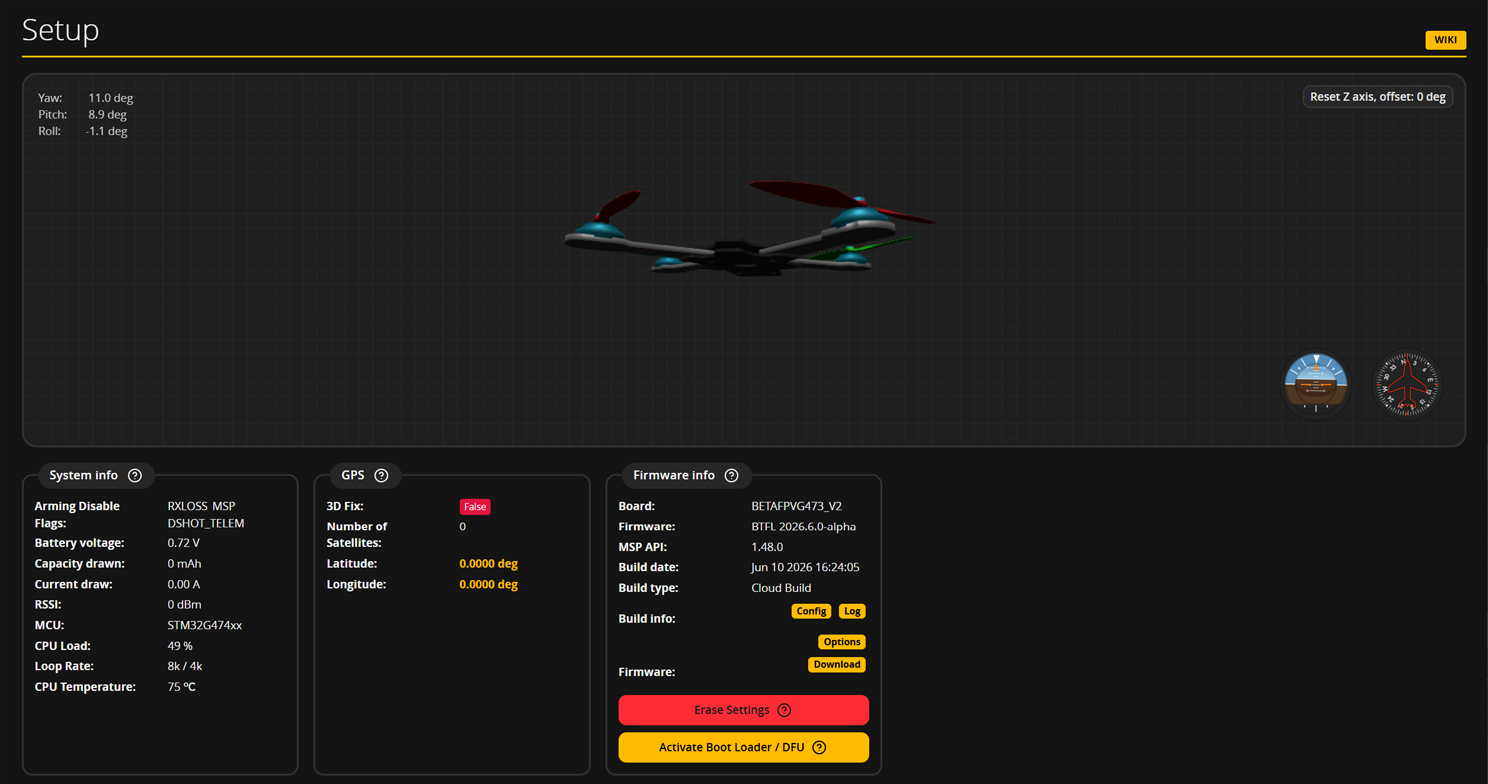
\includegraphics[width=\linewidth]{img/bf-setup.png}\caption{Setup}\end{subfigure}\hfill
\begin{subfigure}[b]{0.49\linewidth}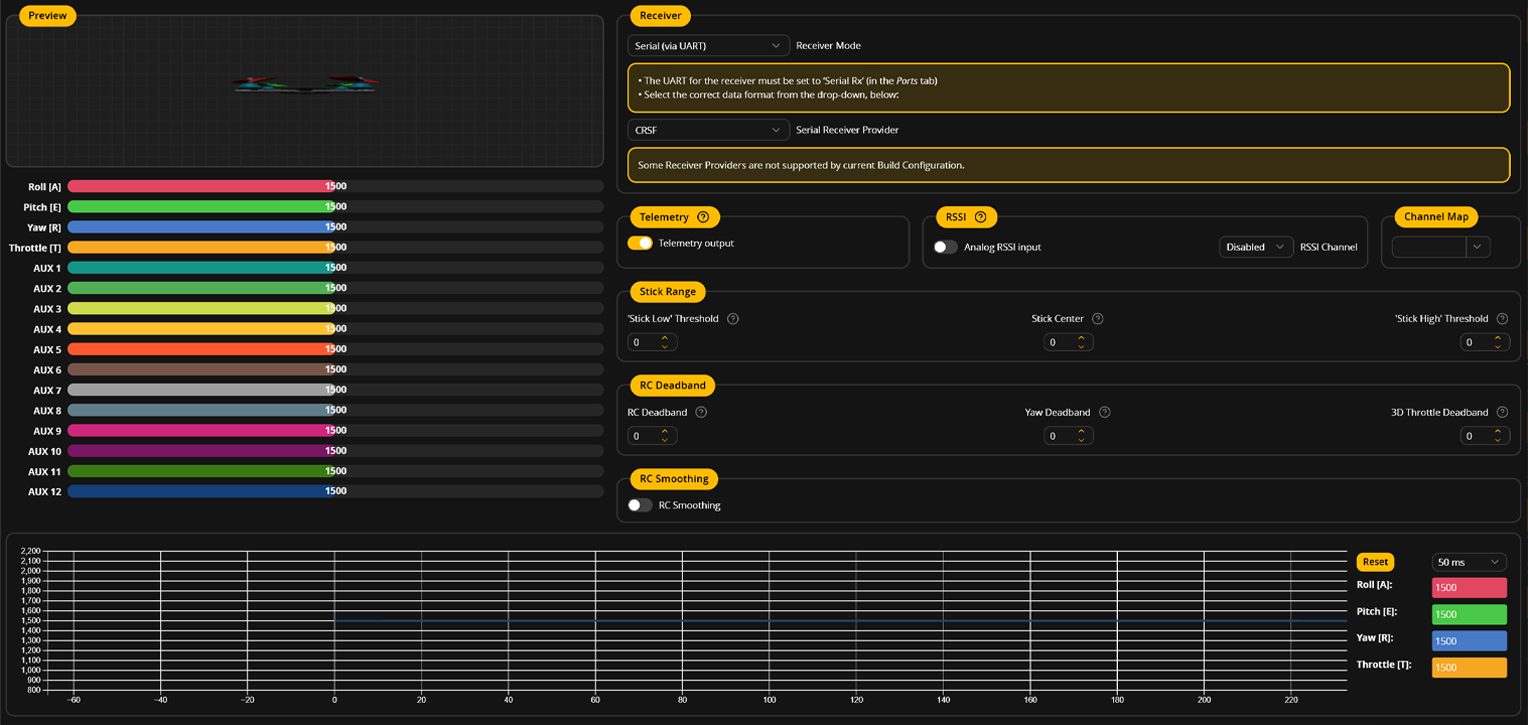
\includegraphics[width=\linewidth]{img/bf-receiver.png}\caption{Receiver}\end{subfigure}\\[2mm]
\begin{subfigure}[b]{0.49\linewidth}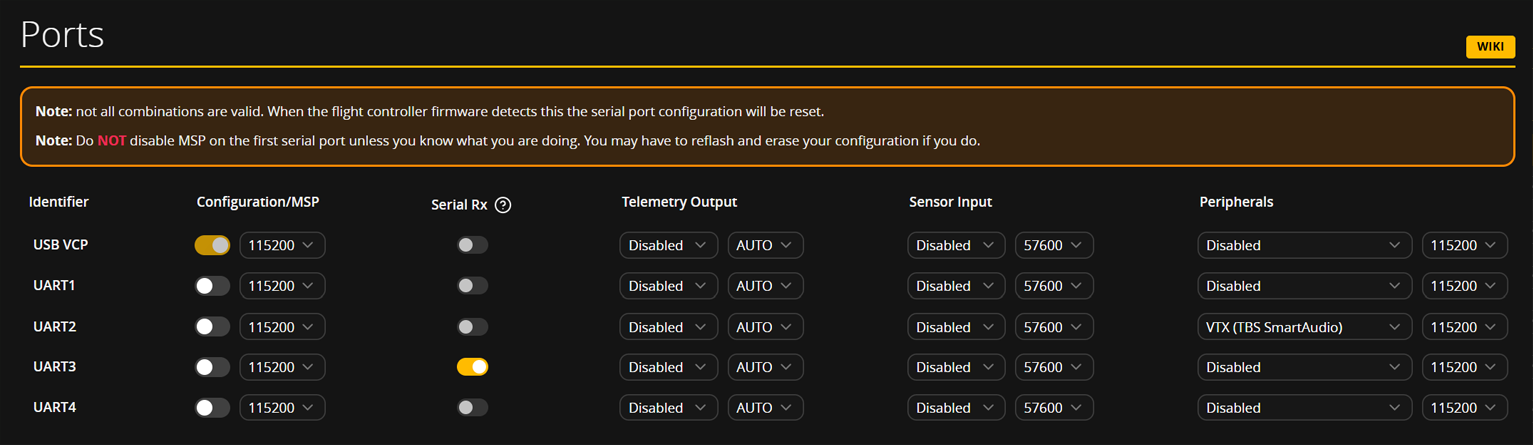
\includegraphics[width=\linewidth]{img/bf-ports.png}\caption{Ports — назначение UART}\end{subfigure}\hfill
\begin{subfigure}[b]{0.49\linewidth}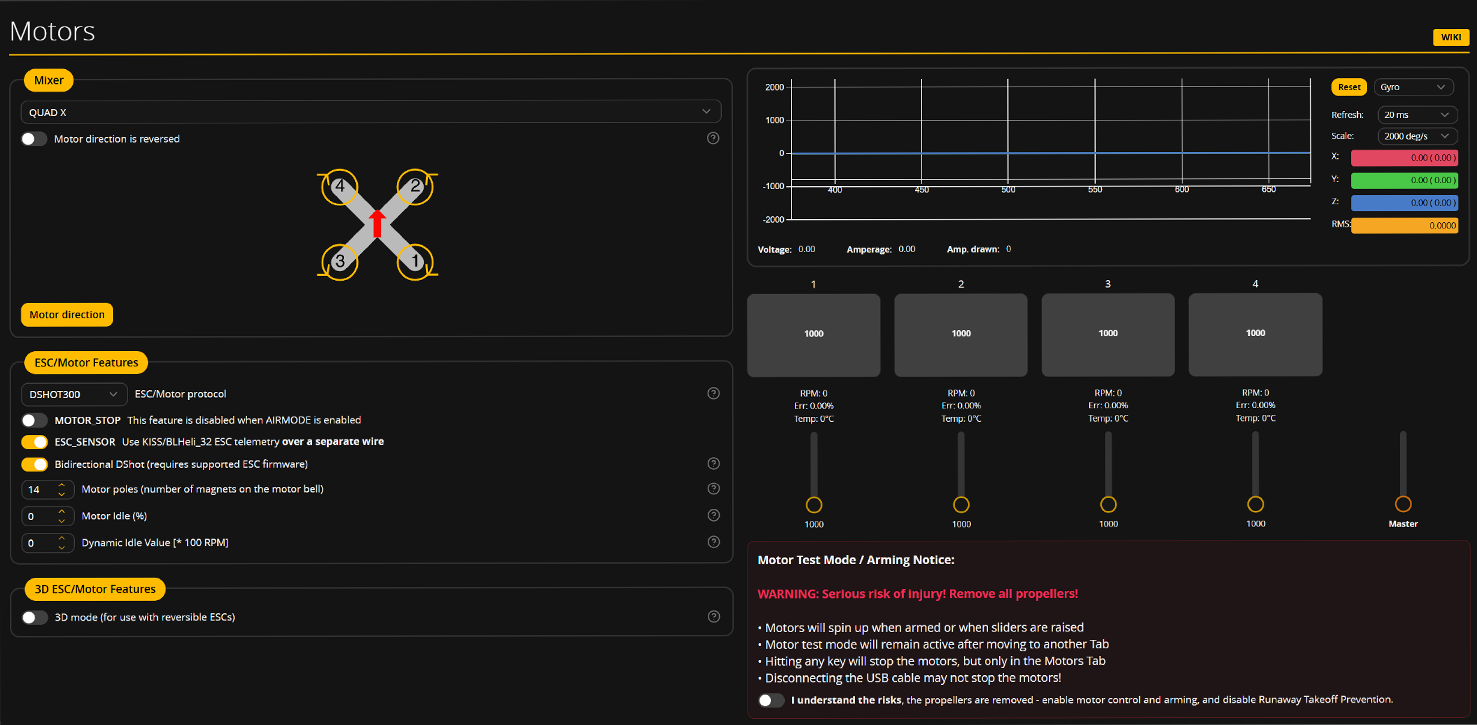
\includegraphics[width=\linewidth]{img/bf-motors.png}\caption{Motors — проверка моторов}\end{subfigure}
\caption{Betaflight Configurator {\color{gray}\scriptsize(скриншоты: документация Betaflight, betaflight.com)}}
\end{figure}

\subsection{INAV}
\begin{itemize}
\item \textbf{Назначение}: навигация. Форк Cleanflight с упором на GPS. Поддерживает мультикоптеры, \textbf{самолёты и летающие крылья}, VTOL, роверы, лодки.
\item Режимы: \term{Position Hold}, \term{Altitude Hold}, \term{RTH} (возврат домой), \term{Waypoint}-миссии (полёт по точкам), Cruise, Loiter, Launch (запуск с руки для самолёта), автопосадка.
\item Программа: \textbf{INAV Configurator} (интерфейс похож на Betaflight) + планировщик миссий, \term{Programming Framework} (логические условия прямо в прошивке), mixer profiles для VTOL.
\item Требует GPS, компас (для коптеров) и барометр. Работает на тех же платах F4/F7/H7, что и Betaflight.
\end{itemize}

\subsection{ArduPilot}
\begin{itemize}
\item \textbf{Назначение}: профессиональный открытый автопилот. Прошивки: \textbf{ArduCopter}, \textbf{ArduPlane} (включая QuadPlane/VTOL), \textbf{Rover}, \textbf{ArduSub} (подводные), \textbf{AntennaTracker}, Blimp.
\item Работает на Pixhawk/Cube, Matek H743 и других H7/F7-платах, а также на Linux (Raspberry Pi, Navio).
\item Протокол \term{MAVLink} — телеметрия и команды. Фильтр Калмана \term{EKF3} для оценки положения.
\item Наземные станции: \textbf{Mission Planner} (Windows), \textbf{QGroundControl} (все ОС и Android), MAVProxy (консоль).
\item Возможности: 20+ режимов (Stabilize, AltHold, Loiter, Auto, RTL, Guided, Land, SmartRTL\ldots), сложные миссии, геозоны, парашют, обход препятствий, скрипты на \textbf{Lua}, компаньон-компьютер (ROS), DroneCAN, резервирование датчиков.
\end{itemize}

\begin{figure}[H]\centering
\begin{subfigure}[b]{0.49\linewidth}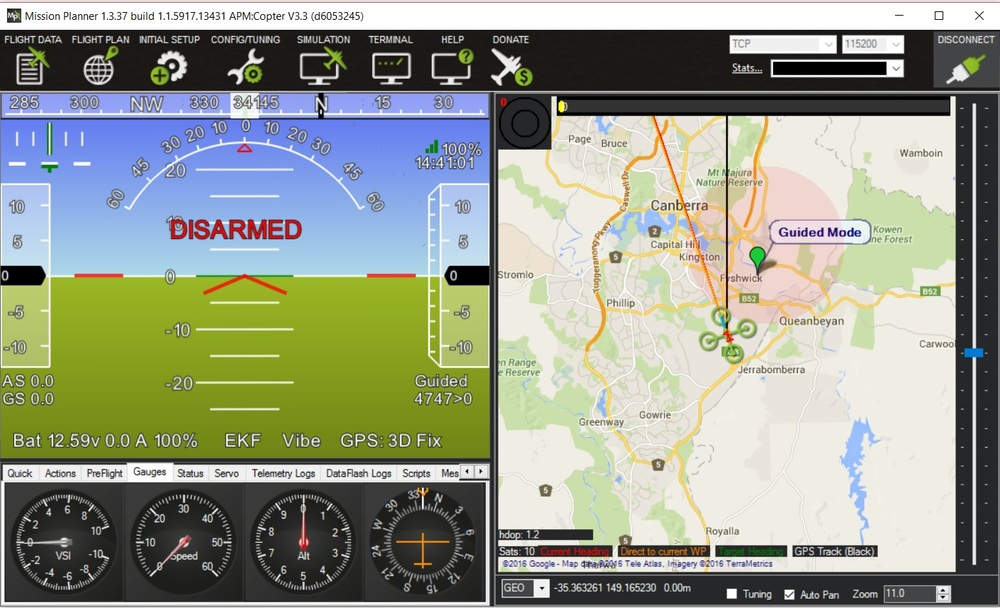
\includegraphics[width=\linewidth]{img/mp-data.jpg}\caption{Flight Data — авиагоризонт и карта}\end{subfigure}\hfill
\begin{subfigure}[b]{0.49\linewidth}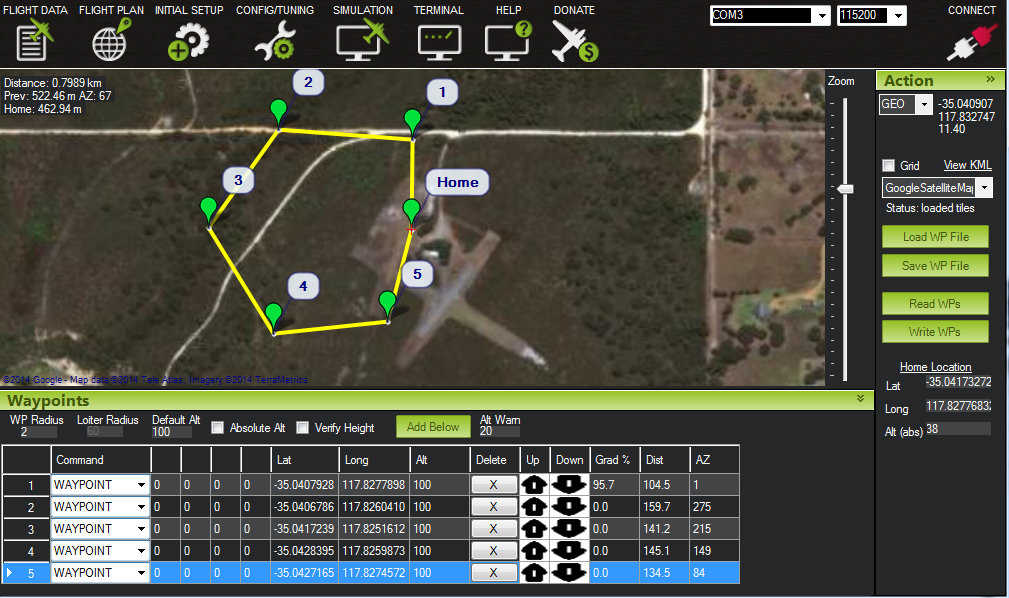
\includegraphics[width=\linewidth]{img/mp-plan.jpg}\caption{Flight Plan — планирование миссии}\end{subfigure}
\caption{Mission Planner для ArduPilot {\color{gray}\scriptsize(скриншоты: ArduPilot Wiki)}}
\end{figure}

\subsection{Сравнение}
\begin{table}[H]\centering\small
\renewcommand{\arraystretch}{1.3}
\begin{tabularx}{\linewidth}{@{}p{28mm} X X X@{}}
\toprule
 & \textbf{Betaflight} & \textbf{INAV} & \textbf{ArduPilot} \\
\midrule
Для чего & FPV, гонки, фристайл & FPV-дальнолёты, самолёты, навигация & Автономные миссии, коммерческие и научные задачи \\
Типы БВС & мультикоптеры & коптеры, самолёты, крылья, VTOL & всё: коптер, самолёт, VTOL, вертолёт, ровер, лодка, подлодка \\
GPS-функции & только GPS Rescue & удержание, RTH, миссии & полный набор + геозоны \\
ПО & Betaflight Configurator & INAV Configurator & Mission Planner, QGroundControl \\
Протокол & MSP & MSP (+ MAVLink телеметрия) & MAVLink \\
Сложность & низкая & средняя & высокая (сотни параметров) \\
Железо & F4/F7/H7 FPV-платы & F4/F7/H7 FPV-платы & Pixhawk, Cube, H7-платы \\
\bottomrule
\end{tabularx}
\caption{Betaflight, INAV, ArduPilot}
\end{table}

\subsection{Вспомогательное ПО}
\begin{itemize}
\item \textbf{ESC Configurator} (веб), \textbf{BLHeliSuite32}, \textbf{AM32 Configurator} — прошивка и настройка регуляторов.
\item \textbf{ExpressLRS Configurator} — прошивка приёмников и модулей ELRS (или через Wi-Fi прямо с устройства).
\item \textbf{EdgeTX / OpenTX} + \textbf{EdgeTX Companion} — прошивка пультов (моделей, микшеров, Lua-скриптов).
\item \textbf{Blackbox Explorer}, \textbf{PID Toolbox} — анализ логов; \textbf{симуляторы}: Liftoff, VelociDrone, Uncrashed, DRL — тренировка без риска.
\end{itemize}

\begin{keybox}[Типичный порядок настройки нового FPV-дрона в Betaflight]
Прошить ПК (Firmware Flasher) $\to$ Setup: калибровка акселерометра $\to$ Ports: включить Serial RX на UART приёмника $\to$ Configuration: протокол ESC (DShot600), ориентация $\to$ Receiver: протокол CRSF, проверить каналы и порядок AETR $\to$ Modes: ARM на тумблере $\to$ Motors: проверить порядок и направление вращения (\textbf{без пропеллеров!}) $\to$ Failsafe $\to$ OSD и VTX $\to$ пробный полёт.
\end{keybox}

\begin{exam}
\begin{enumerate}
\item Какую прошивку выбрать для гоночного дрона, для крыла-дальнолёта, для картографирования по миссии?
\item Что такое режим Acro и чем он отличается от Angle?
\item Что такое MAVLink? Какие наземные станции вы знаете?
\end{enumerate}
\end{exam}

\section{Протоколы передачи: UART, PWM, PPM, SBUS}

Протоколы нужны, чтобы передавать команды \textbf{от приёмника к полётному контроллеру} и \textbf{от контроллера к регуляторам/сервоприводам}, а также связывать ПК с периферией (GPS, VTX, телеметрия).

\begin{figure}[H]\centering
\begin{tikzpicture}[font=\sffamily\small,node distance=24mm]
\node[blk,fill=blk3] (tx) {Пульт};
\node[blk,fill=blk2,right=of tx] (rx) {Приёмник};
\node[blk,fill=blk1,right=of rx] (fc) {Полётный\\контроллер};
\node[blk,fill=blk4,right=of fc] (esc) {ESC\,/\,сервы};
\draw[arr,decorate,decoration={snake,amplitude=.8mm,segment length=4mm,post length=2mm}] (tx) -- node[above,font=\scriptsize]{радио} (rx);
\draw[arr] (rx) -- node[above,font=\scriptsize]{PWM, PPM,} node[below,font=\scriptsize]{SBUS, CRSF} (fc);
\draw[arr] (fc) -- node[above,font=\scriptsize]{PWM, OneShot,} node[below,font=\scriptsize]{DShot} (esc);
\end{tikzpicture}
\caption{Где какие протоколы используются}
\end{figure}

\subsection{UART — универсальный асинхронный приёмопередатчик}
\begin{itemize}
\item Аппаратный интерфейс микроконтроллера, на котором работает большинство «серийных» протоколов (SBUS, CRSF, IBUS, GPS, MSP, MAVLink, SmartAudio).
\item Линии: \textbf{TX} (передача), \textbf{RX} (приём), \textbf{GND}. Подключение \textbf{крест-накрест}: TX одного устройства $\to$ RX другого. Двусторонний (full duplex).
\item \term{Асинхронный} — нет отдельной линии тактирования, обе стороны заранее договариваются о \term{скорости} (baud rate): 9600, 57600, 115200, 420000 бод\ldots
\item Кадр: в покое линия в «1» $\to$ \textbf{стартовый бит} «0» $\to$ 8 бит данных (младший первым) $\to$ [бит чётности] $\to$ \textbf{стоповый бит(ы)} «1». Формат записывают как \code{8N1} (8 бит, без чётности, 1 стоп) или \code{8E2}.
\end{itemize}

\begin{figure}[H]\centering
\begin{tikzpicture}[x=9mm,y=7mm,font=\sffamily\scriptsize]
\draw[very thick,accent] (0,1) -- (1,1) -- (1,0) -- (2,0) -- (2,1) -- (3,1) -- (3,0) -- (8,0) -- (8,1) -- (9,1) -- (9,0) -- (10,0) -- (10,1) -- (12,1);
\foreach \x in {1,...,11} \draw[gray!50,dashed] (\x,-0.2) -- (\x,1.3);
\node at (0.5,1.5) {покой};
\node at (1.5,1.5) {\textbf{старт}};
\foreach \i/\b in {0/1,1/0,2/0,3/0,4/0,5/0,6/1,7/0} \node at (2.5+\i,1.5) {D\i};
\foreach \i/\b in {0/1,1/0,2/0,3/0,4/0,5/0,6/1,7/0} \node[text=gray] at (2.5+\i,-0.45) {\b};
\node at (10.5,1.5) {\textbf{стоп}};
\node at (11.5,1.5) {покой};
\draw[decorate,decoration={brace,mirror,amplitude=4pt}] (2,-0.8) -- (10,-0.8) node[midway,below=4pt] {байт 0x41 = «A», младший бит первым};
\end{tikzpicture}
\caption{Кадр UART 8N1 для символа «A»}
\end{figure}

\photo{0.45\linewidth}{runcam.jpg}{Подключение устройства к ПК по UART: TX $\to$ RX, RX $\to$ TX, общий GND}{ArduPilot Wiki}

\subsection{PWM — широтно-импульсная модуляция}
\begin{itemize}
\item Самый старый способ: \textbf{один провод на каждый канал}. Значение канала кодируется \textbf{длительностью импульса}: \SI{1000}{\micro\second} — минимум, \SI{1500}{\micro\second} — центр, \SI{2000}{\micro\second} — максимум.
\item Период — \SI{20}{\milli\second} (частота \SI{50}{\hertz}) для аналоговых сервоприводов, до 400--490~Гц для ESC.
\item Минусы: много проводов (8 каналов — 8 сигнальных проводов), медленно, нет телеметрии. Сегодня — только для серв и простых самолётов.
\end{itemize}

\begin{figure}[H]\centering
\begin{tikzpicture}[x=5mm,y=6mm,font=\sffamily\scriptsize]
\draw[->] (0,0) -- (25,0) node[right] {$t$};
\draw[very thick,accent] (0,0) -- (1,0) -- (1,1) -- (2,1) -- (2,0) -- (11,0) -- (11,1) -- (12.5,1) -- (12.5,0) -- (21,0) -- (21,1) -- (23,1) -- (23,0) -- (24,0);
\node[above] at (1.5,1) {1000\,мкс};
\node[above] at (11.75,1) {1500\,мкс};
\node[above] at (22,1) {2000\,мкс};
\node[below] at (1.5,0) {минимум};
\node[below] at (11.75,0) {центр};
\node[below] at (22,0) {максимум};
\draw[<->] (1,-1.1) -- node[below] {период 20\,мс (50\,Гц)} (11,-1.1);
\end{tikzpicture}
\caption{Сигнал PWM: значение задаётся шириной импульса}
\end{figure}

\subsection{PPM (CPPM) — импульсно-позиционная модуляция}
\begin{itemize}
\item \textbf{Все каналы по одному проводу}, друг за другом. Значение канала — \textbf{интервал между соседними импульсами} (\SIrange{1000}{2000}{\micro\second}).
\item После последнего канала — длинная пауза (> \SI{3}{\milli\second}) для синхронизации. Кадр $\approx$ \SI{22.5}{\milli\second}, обычно \textbf{до 8 каналов}.
\item Плюс — один провод. Минусы — мало каналов, большая задержка, чувствительность к джиттеру. Сегодня устарел.
\end{itemize}

\begin{figure}[H]\centering
\begin{tikzpicture}[x=4mm,y=6mm,font=\sffamily\scriptsize]
\draw[->] (0,0) -- (38,0) node[right] {$t$};
\def\p#1{-- (#1,0) -- (#1,1) -- ({#1+0.4},1) -- ({#1+0.4},0)}
\draw[very thick,accent] (0,0) \p{1} \p{4} \p{7.5} \p{10} \p{13.5} \p{16.5} \p{19} \p{22.5} \p{25} -- (35,0) \p{35} -- (37,0);
\foreach \a/\b/\n in {1/4/1,4/7.5/2,7.5/10/3,10/13.5/4,13.5/16.5/5,16.5/19/6,19/22.5/7,22.5/25/8}
  \draw[<->,gray] (\a,1.4) -- node[above,text=black] {CH\n} (\b,1.4);
\draw[<->] (25,-0.6) -- node[below] {синхропауза} (35,-0.6);
\draw[decorate,decoration={brace,mirror,amplitude=4pt}] (1,-1.4) -- (35,-1.4) node[midway,below=4pt] {один кадр $\approx$ 22,5\,мс};
\end{tikzpicture}
\caption{Сигнал PPM: 8 каналов в одном проводе}
\end{figure}

\begin{figure}[H]\centering
\begin{minipage}{0.46\linewidth}\centering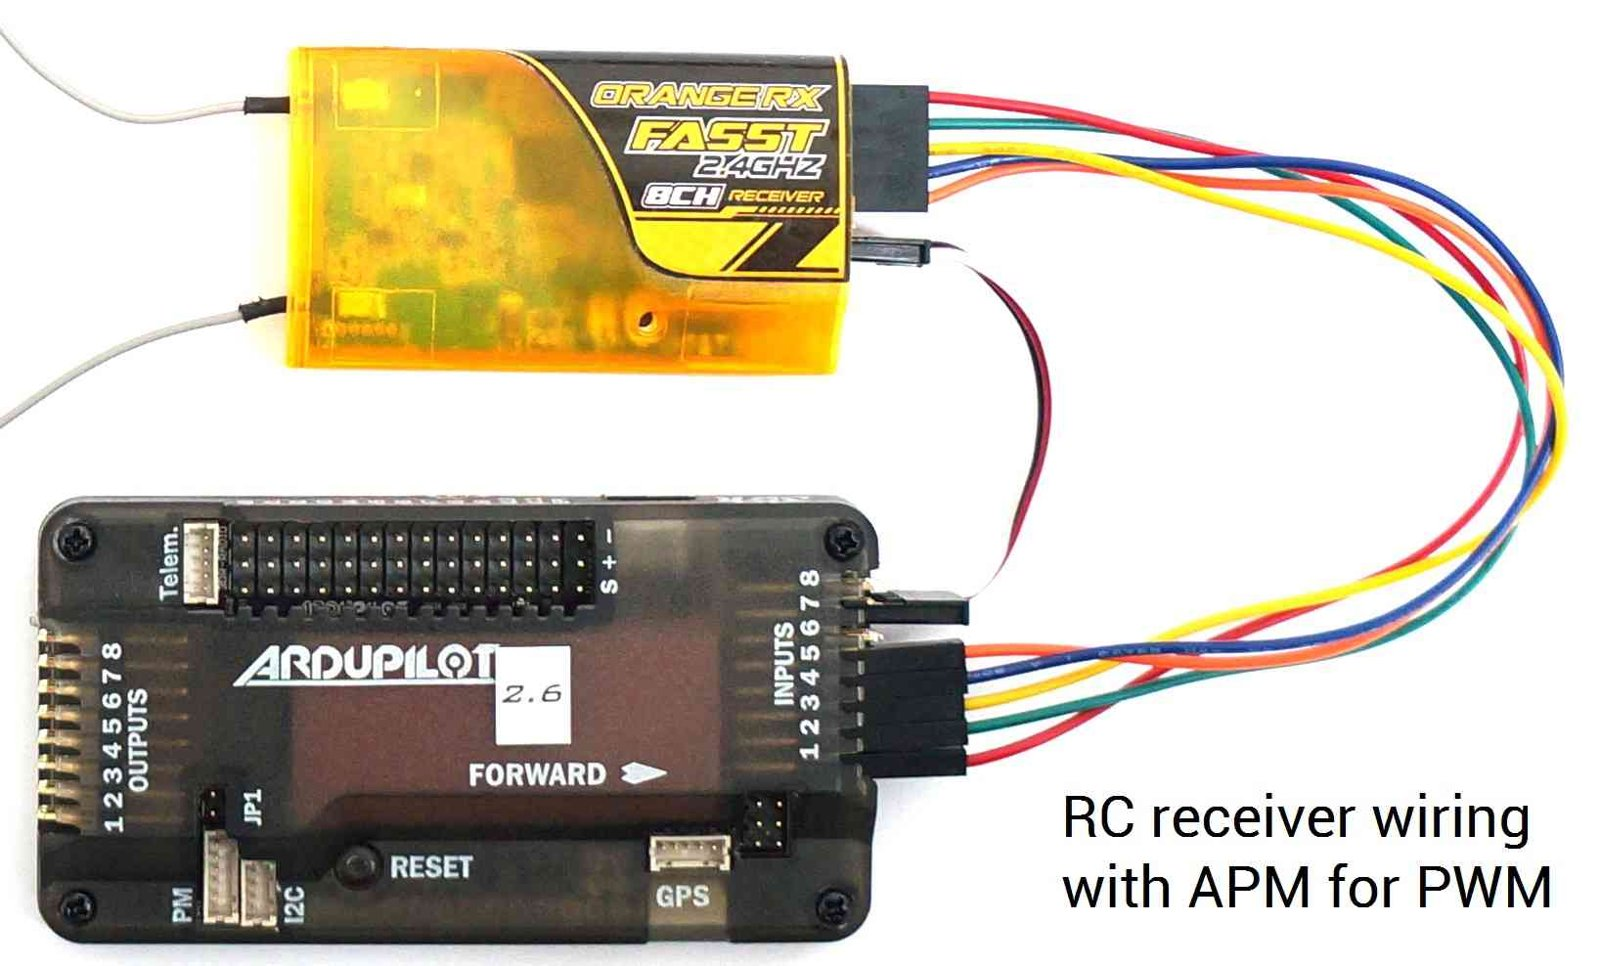
\includegraphics[width=\linewidth]{img/pwm-wiring.jpg}\\{\small PWM: отдельный провод на каждый канал}\end{minipage}\hfill
\begin{minipage}{0.46\linewidth}\centering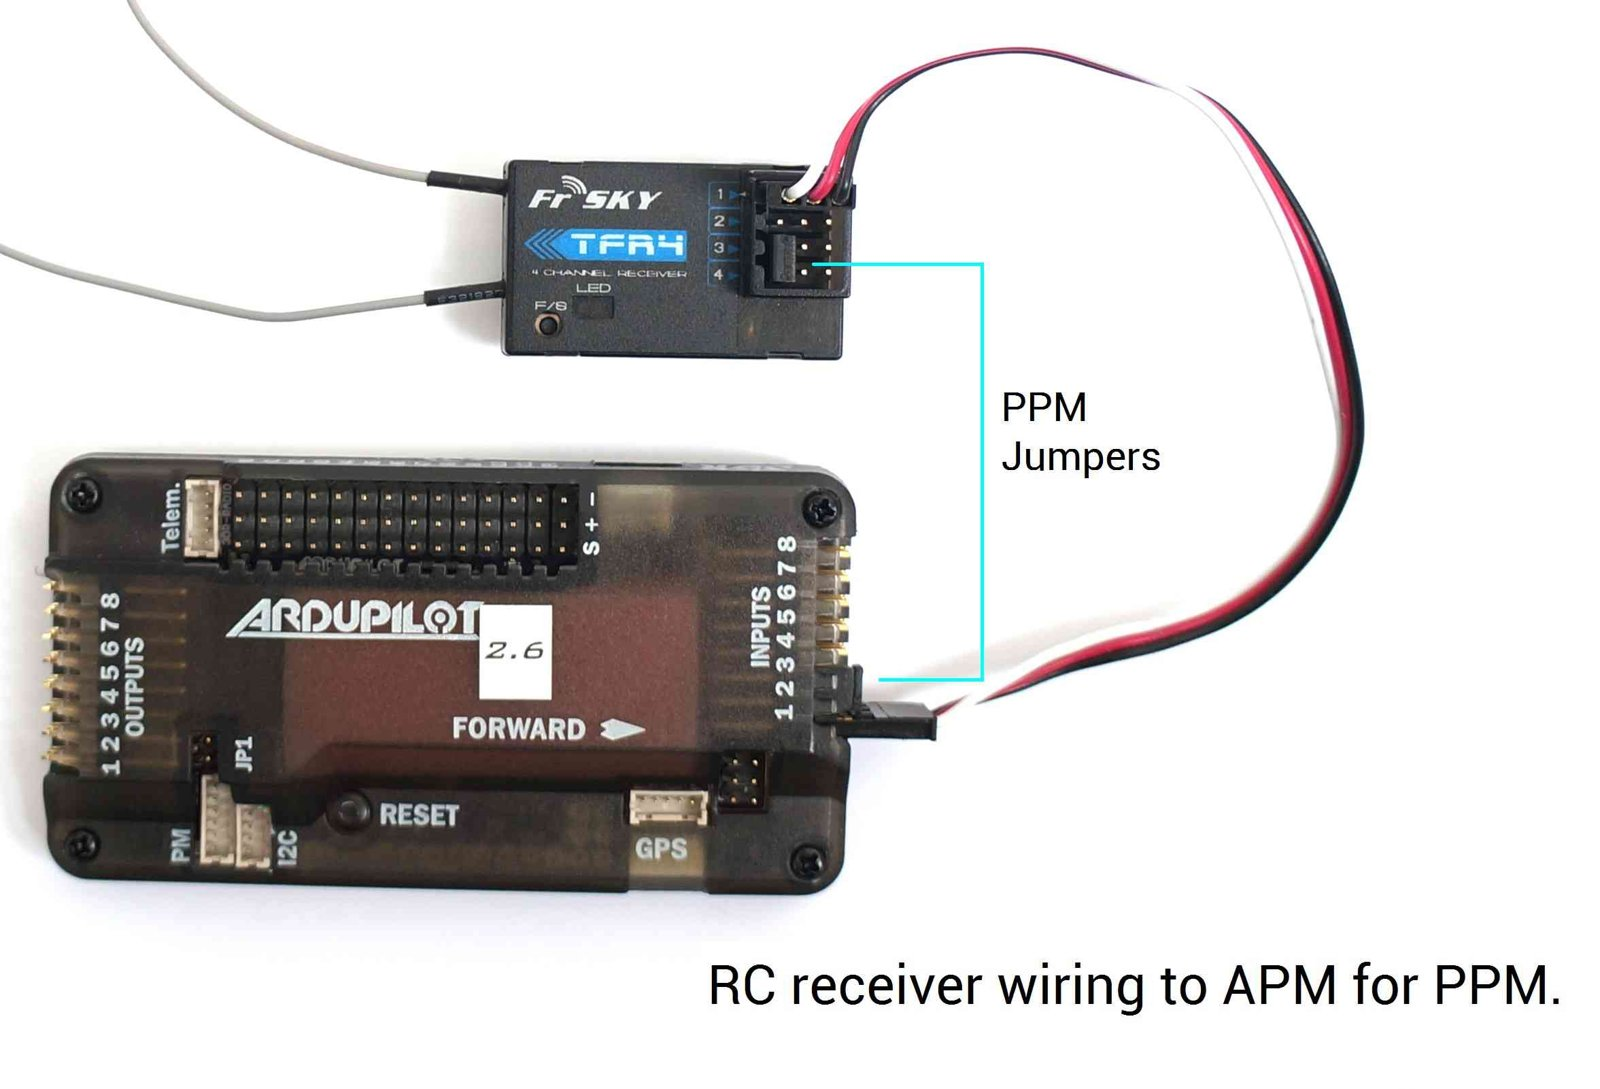
\includegraphics[width=\linewidth]{img/ppm-wiring.jpg}\\{\small PPM: все каналы по одному проводу}\end{minipage}
\caption{Подключение приёмника по PWM и PPM {\color{gray}\scriptsize(фото: ArduPilot Wiki)}}
\end{figure}

\subsection{SBUS (Futaba S.BUS)}
\begin{itemize}
\item \textbf{Цифровой последовательный} протокол поверх UART, разработан Futaba, широко применяется FrSky и другими.
\item Параметры UART: \SI{100000}{бод}, \code{8E2} (чётность even, 2 стоп-бита), \textbf{инвертированный сигнал} — поэтому на F4-контроллерах нужен специальный вход с инвертором (на F7/H7 инверсия есть в самом UART).
\item Кадр \textbf{25 байт}: заголовок \code{0x0F} + 22 байта данных (\textbf{16 каналов по 11 бит}, значения 0–2047) + байт флагов (2 цифровых канала, \textbf{frame lost}, \textbf{failsafe}) + конец \code{0x00}. Кадр каждые \SI{14}{\milli\second} (или 7~мс в быстром режиме).
\item Только в одну сторону. Телеметрию FrSky передаёт отдельно по \textbf{S.Port} или совмещённо в протоколе \textbf{FPort}.
\end{itemize}

\begin{figure}[H]\centering
\begin{tikzpicture}[font=\sffamily\scriptsize,x=5.9mm,y=7mm]
\draw[fill=blk4] (0,0) rectangle (2,1) node[midway] {0x0F};
\draw[fill=blk1] (2,0) rectangle (24,1) node[midway] {22 байта = 16 каналов × 11 бит};
\draw[fill=blk3] (24,0) rectangle (26,1) node[midway] {флаги};
\draw[fill=blk4] (26,0) rectangle (28,1) node[midway] {0x00};
\node[below] at (1,0) {заголовок}; \node[below] at (25,0) {ch17,18, FS}; \node[below] at (27,0) {конец};
\end{tikzpicture}
\caption{Кадр SBUS (25 байт)}
\end{figure}

\subsection{Другие протоколы (полезно знать)}
\begin{table}[H]\centering\small
\renewcommand{\arraystretch}{1.25}
\begin{tabularx}{\linewidth}{@{}p{24mm} X@{}}
\toprule
\textbf{CRSF} & Протокол TBS Crossfire, используется и в \textbf{ELRS}. UART \SI{420000}{бод} \code{8N1}, не инвертирован, до 16 каналов, \textbf{двусторонний}: телеметрия (RSSI, LQ, напряжение, GPS) идёт обратно в пульт. Кадр: \code{[0xC8][длина][тип][данные][CRC8]}. Сейчас — стандарт де-факто. \\
\textbf{IBUS} & FlySky, UART 115200 бод, 32-байтный кадр, 14 каналов. \\
\textbf{FPort} & FrSky: SBUS + S.Port-телеметрия в одном проводе. \\
\textbf{DSM/DSMX} & Spektrum, спутниковые приёмники по UART. \\
\textbf{MSP} & MultiWii Serial Protocol — обмен ПК с конфигуратором, OSD в цифровых очках (MSP DisplayPort), VTX. \\
\textbf{MAVLink} & Телеметрия и команды ArduPilot/PX4 $\leftrightarrow$ наземная станция. \\
\textbf{I$^2$C, SPI, CAN} & Внутренние шины: SPI — гироскоп, OSD, флеш; I$^2$C — компас, барометр, дисплей; CAN (DroneCAN) — GPS, ESC, датчики на ArduPilot. \\
\bottomrule
\end{tabularx}
\caption{Другие протоколы связи}
\end{table}

\subsection{Протоколы ПК $\to$ ESC}
\begin{table}[H]\centering\small
\begin{tabular}{@{}llll@{}}
\toprule
\textbf{Протокол} & \textbf{Тип} & \textbf{Длительность / скорость} & \textbf{Особенность} \\
\midrule
PWM & аналоговый & 1000–2000 мкс & нужна калибровка ESC \\
OneShot125 & аналоговый & 125–250 мкс & в 8 раз быстрее PWM \\
OneShot42 / MultiShot & аналоговый & 42–84 / 5–25 мкс & ещё быстрее \\
\textbf{DShot150/300/600} & \textbf{цифровой} & 150/300/600 кбит/с & без калибровки, CRC, команды \\
Bidirectional DShot & цифровой & — & обратно — обороты (RPM-фильтр) \\
\bottomrule
\end{tabular}
\caption{Протоколы управления регуляторами}
\end{table}
\textbf{Кадр DShot — 16 бит}: 11 бит газа (0 — стоп, 1–47 — команды, 48–2047 — газ), 1 бит запроса телеметрии, 4 бита контрольной суммы. «1» и «0» различаются длительностью высокого уровня внутри бита.

\begin{exam}
\begin{enumerate}
\item Как в PWM кодируется значение канала? А в PPM?
\item Сколько каналов у SBUS, какова скорость и почему на F4 нужен инвертор?
\item Как подключается UART-устройство к ПК? Что означает запись 8N1?
\item Чем DShot лучше PWM для управления моторами?
\end{enumerate}
\end{exam}

\section{Системы управления: ELRS, FrSky и другие}

\subsection{Из чего состоит радиоуправление}
\begin{itemize}
\item \term{Пульт} (аппаратура, «радио») — стики, тумблеры, экран. Прошивка — обычно \textbf{EdgeTX} (открытая, наследник OpenTX). Модели: RadioMaster TX16S, Boxer, Zorro, Pocket; FrSky Taranis; TBS Tango 2; Jumper.
\item \term{Передающий модуль} (TX) — встроенный в пульт или внешний в отсек \textbf{JR} (большой) / \textbf{Nano} (Lite).
\item \term{Приёмник} (RX) на борту — связан с ПК по CRSF/SBUS/IBUS.
\item \term{Привязка} (bind) — пара «передатчик–приёмник» запоминают друг друга, чтобы не реагировать на чужие пульты.
\item \term{FHSS} — псевдослучайная перестройка частоты десятки–сотни раз в секунду: устойчивость к помехам и совместная работа многих пилотов.
\item \term{Failsafe} — поведение при потере связи: отключить моторы (drop), удерживать последние значения (hold) или возврат домой (RTH, GPS Rescue).
\item \term{RSSI} — уровень сигнала (дБм); \term{LQ} (Link Quality) — процент успешно принятых пакетов. LQ важнее RSSI.
\end{itemize}

\begin{figure}[H]\centering
\begin{minipage}[b]{0.30\linewidth}\centering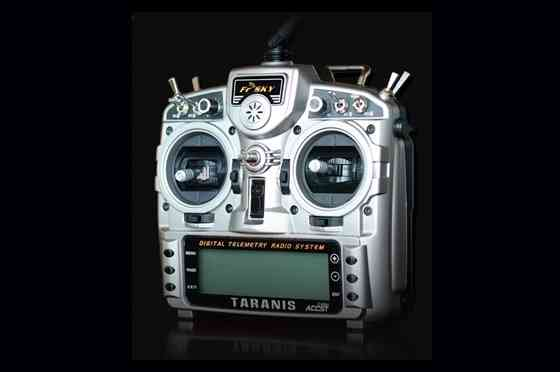
\includegraphics[width=\linewidth]{img/taranis.jpg}\\{\small FrSky Taranis}\end{minipage}\hfill
\begin{minipage}[b]{0.34\linewidth}\centering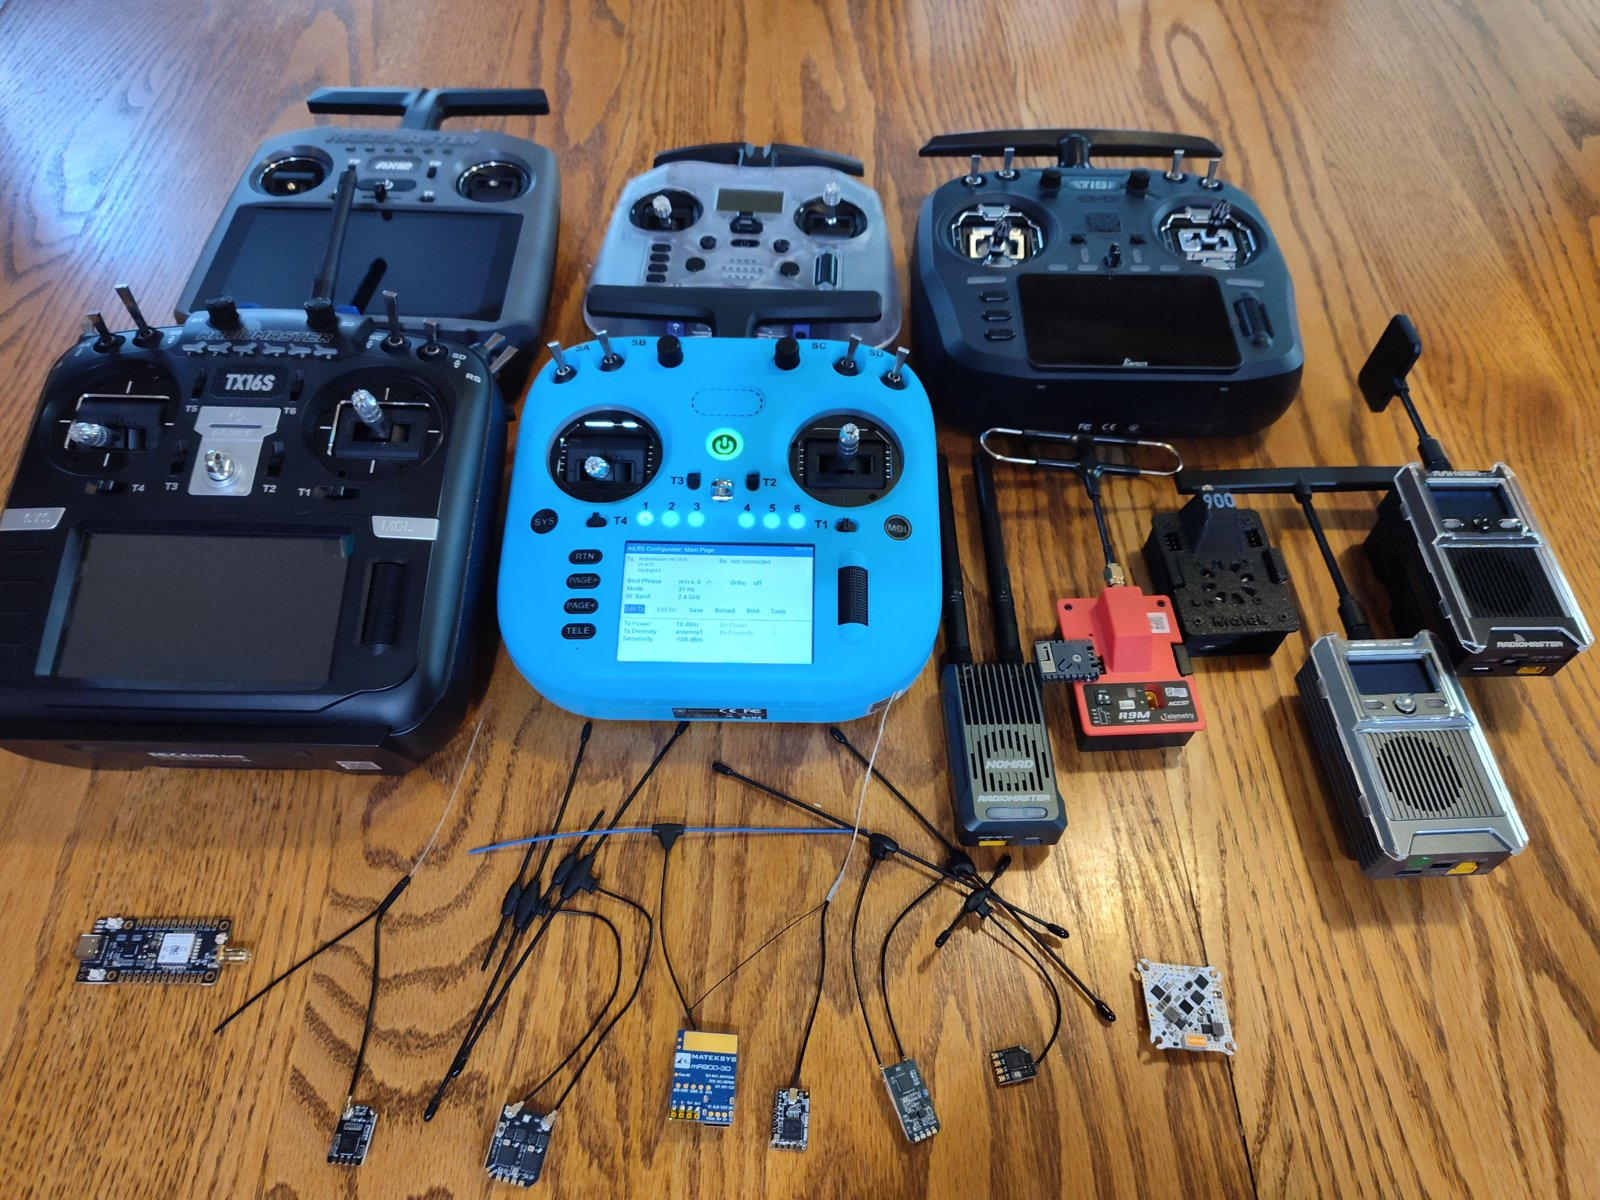
\includegraphics[width=\linewidth]{img/mlrs.jpg}\\{\small Пульты и модули на EdgeTX}\end{minipage}\hfill
\begin{minipage}[b]{0.30\linewidth}\centering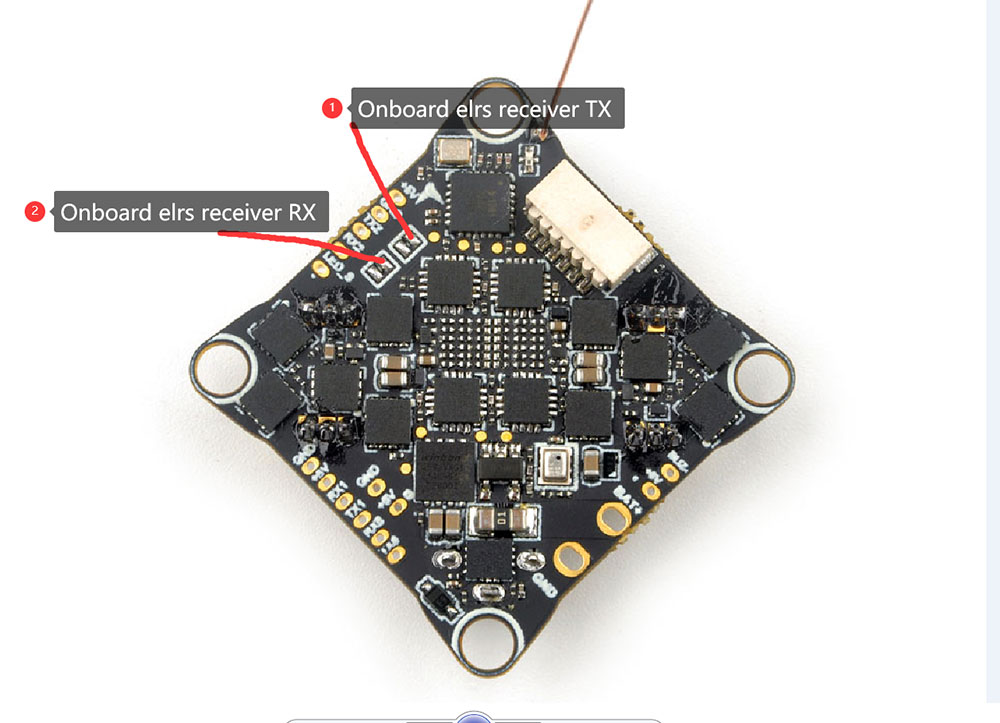
\includegraphics[width=\linewidth]{img/elrs-ext.jpg}\\{\small Приёмник ELRS на полётном контроллере}\end{minipage}
\caption{Аппаратура управления и приёмники {\color{gray}\scriptsize(фото: ArduPilot Wiki)}}
\end{figure}

\subsection{ExpressLRS (ELRS)}
\begin{itemize}
\item \textbf{Открытый} (open source) проект, появился в 2020 г. Сейчас — самый популярный RC-линк в FPV. Дешёвое железо многих производителей (RadioMaster, BetaFPV, HappyModel\ldots).
\item Радиочипы Semtech: \textbf{SX1280} (\SI{2.4}{\giga\hertz}), \textbf{SX1276} (\SIrange{868}{915}{\mega\hertz}), \textbf{LR1121} (двухдиапазонный).
\item Модуляции: \term{LoRa} (большая чувствительность — дальность) и \term{FLRC} (высокая скорость — малая задержка).
\item \term{Частота пакетов} (packet rate): от 25–50~Гц (максимальная дальность) до 500 Гц и \textbf{F1000} (1000 пакетов/с, минимальная задержка для гонок). \textbf{Чем выше частота пакетов — тем меньше задержка, но меньше дальность.}
\item Мощность: \SIrange{10}{1000}{\milli\watt} (некоторые модули — до 2~Вт), \term{динамическая мощность} — снижается, когда сигнал хороший.
\item \term{Binding phrase} — привязка по общей «фразе» в прошивке вместо нажатия кнопок. Обновление по Wi-Fi прямо с приёмника.
\item Протокол к ПК — \textbf{CRSF}, двусторонняя телеметрия (RSSI, LQ, батарея, GPS). Режим \textbf{Gemini} — одновременная передача на двух частотах/антеннах для надёжности; двухдиапазонные приёмники (2,4\,ГГц + 900\,МГц).
\end{itemize}

\subsection{TBS Crossfire и Tracer}
\begin{itemize}
\item \textbf{Crossfire} (Team BlackSheep, 2016) — закрытая система \SIrange{868}{915}{\mega\hertz}, мощность до 2~Вт, частота 50/150~Гц, дальность десятки километров. Именно в нём появился протокол \textbf{CRSF}. Долго был «золотым стандартом» дальнолётов.
\item \textbf{Tracer} — вариант на \SI{2.4}{\giga\hertz} с меньшей задержкой (250~Гц).
\end{itemize}

\subsection{FrSky}
\begin{itemize}
\item Протоколы: \textbf{ACCST D8} (8 каналов, старый), \textbf{ACCST D16} (16 каналов), \textbf{ACCESS} (с 2019, до 24 каналов, новая привязка), \textbf{TANDEM} (одновременно 900~МГц и 2,4~ГГц), \textbf{R9} (900~МГц, дальнолёты).
\item Приёмники: XM+, R-XSR, Archer, X8R; выход \textbf{SBUS}, телеметрия \textbf{S.Port}, совмещённый \textbf{FPort}.
\item Пульты Taranis X9D, X-Lite, Horus. Долгое время был стандартом в FPV, сейчас вытесняется ELRS (закрытость, несовместимость версий прошивок EU/FCC).
\end{itemize}

\subsection{Другие системы}
\begin{table}[H]\centering\small
\renewcommand{\arraystretch}{1.25}
\begin{tabularx}{\linewidth}{@{}p{30mm} X@{}}
\toprule
\textbf{FlySky} & AFHDS 2A, AFHDS 3, протокол \textbf{IBUS}. Дешёвые наборы для начинающих. \\
\textbf{Spektrum} & DSM2/DSMX, популярен у авиамоделистов (самолёты, вертолёты) в США. \\
\textbf{Futaba} & FASST, S-FHSS, T-FHSS; изобретатель \textbf{SBUS}. Профессиональные авиамодели. \\
\textbf{Radiolink} & Бюджетные системы, свои протоколы, SBUS/PPM. \\
\textbf{mLRS} & Открытый дальнобойный линк для \textbf{MAVLink} (ArduPilot): управление + полноценная телеметрия в одном канале. \\
\textbf{SiK / RFD900} & Модемы телеметрии MAVLink 433/868/915~МГц для наземной станции. \\
\textbf{DJI} & В экосистеме DJI управление и видео идут в одном цифровом канале (OcuSync). \\
\bottomrule
\end{tabularx}
\caption{Прочие системы связи}
\end{table}

\begin{figure}[H]\centering
\begin{minipage}[b]{0.38\linewidth}\centering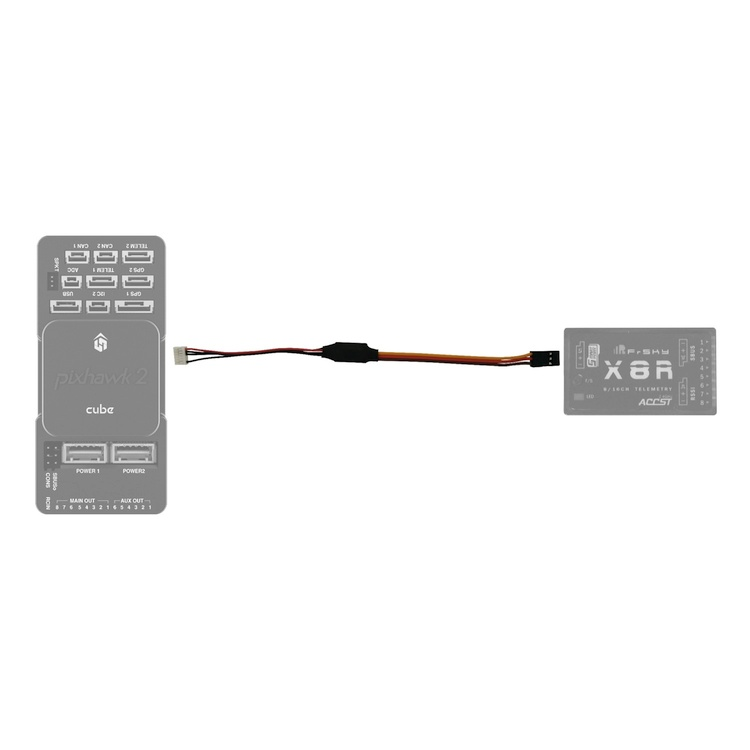
\includegraphics[width=\linewidth]{img/frsky-x8r.jpg}\\{\small Приёмник FrSky и полётный контроллер}\end{minipage}\hspace{1cm}
\begin{minipage}[b]{0.34\linewidth}\centering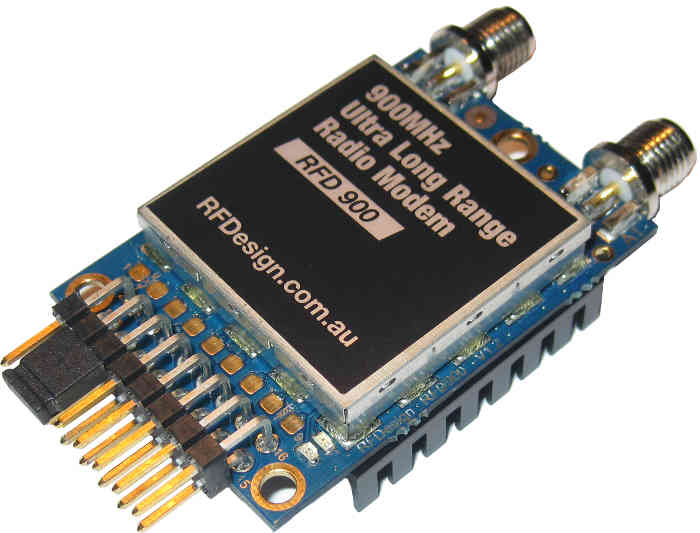
\includegraphics[width=\linewidth]{img/rfd900.jpg}\\{\small Модем телеметрии RFD900}\end{minipage}
\caption{Приёмник и модем телеметрии {\color{gray}\scriptsize(фото: ArduPilot Wiki)}}
\end{figure}

\subsection{Сравнение по частотам}
\begin{table}[H]\centering\small
\renewcommand{\arraystretch}{1.25}
\begin{tabularx}{\linewidth}{@{}p{25mm} X X@{}}
\toprule
 & \textbf{2,4 ГГц} & \textbf{868/915 МГц} \\
\midrule
Системы & ELRS 2.4, Tracer, FrSky ACCST/ACCESS, FlySky, Spektrum & ELRS 900, Crossfire, FrSky R9, mLRS \\
Задержка & меньше (до 1000 Гц) & больше (25–200 Гц) \\
Дальность & меньше & больше (меньше затухание) \\
Огибание препятствий & хуже & лучше (длиннее волна) \\
Антенны & маленькие (\SI{3}{\centi\metre}) & крупнее (\SI{8}{\centi\metre}, «T»-антенны) \\
Помехи & Wi-Fi, Bluetooth & меньше, но LoRa-устройства, GSM-900 \\
\bottomrule
\end{tabularx}
\caption{2,4 ГГц против 868/915 МГц}
\end{table}

\begin{caution}[Частоты и мощность в России]
Без разрешения можно использовать только устройства в разрешённых полосах и с ограниченной мощностью (решения ГКРЧ; для 868~МГц и 2,4~ГГц — единицы–сотни милливатт в зависимости от полосы). Мощные передатчики (1–2~Вт) и нестандартные частоты требуют разрешения. Диапазон 915~МГц (США) в России не выделен для таких устройств — используйте прошивку/регион \textbf{EU 868}.
\end{caution}

\begin{exam}
\begin{enumerate}
\item Почему ELRS вытеснил FrSky? Какие модуляции использует ELRS?
\item Как связаны частота пакетов, задержка и дальность?
\item Что такое failsafe, RSSI и LQ?
\item Чем 900-мегагерцовые системы лучше 2,4 ГГц и чем хуже?
\end{enumerate}
\end{exam}

\section{Дальность связи}

Дальность определяется тем, дойдёт ли до приёмника сигнал, который \textbf{сильнее его порога чувствительности} (и сильнее помех). Это считают через \term{бюджет радиолинии}.

\subsection{Децибелы — быстрая памятка}
\begin{itemize}
\item \term{дБм} — мощность относительно \SI{1}{\milli\watt}: $P_\text{дБм} = 10\lg\frac{P}{1\,\text{мВт}}$. \SI{25}{\milli\watt} = 14~дБм; \SI{100}{\milli\watt} = 20~дБм; \SI{250}{\milli\watt} = 24~дБм; \SI{1}{\watt} = 30~дБм.
\item \textbf{+3~дБ} = мощность ×2; \textbf{+10~дБ} = ×10; \textbf{+6~дБ} = дальность ×2 (в свободном пространстве).
\item \term{дБи} — усиление антенны относительно идеального изотропного излучателя. Диполь — 2~дБи, патч — 8–10~дБи, helical — 10–14~дБи.
\end{itemize}

\subsection{Потери в свободном пространстве и бюджет линии}
\begin{formula}[Потери в свободном пространстве (FSPL)]
\[
L_\text{FSPL}\,[\text{дБ}] = 20\lg d_\text{км} + 20\lg f_\text{МГц} + 32{,}44
\]
Потери растут с \textbf{расстоянием} и с \textbf{частотой}: удвоение расстояния даёт +6~дБ потерь. При одинаковой дальности на 900~МГц потери на $\approx$\,8,5~дБ меньше, чем на 2,4~ГГц.
\end{formula}

\begin{formula}[Бюджет радиолинии]
\[
P_\text{пр} = P_\text{пер} + G_\text{пер} + G_\text{пр} - L_\text{FSPL} - L_\text{доп} \;\geq\; S_\text{пр} + M
\]
$P_\text{пер}$ — мощность передатчика (дБм), $G$ — усиления антенн (дБи), $L_\text{доп}$ — потери в кабелях, на препятствиях, из-за поляризации, $S_\text{пр}$ — \textbf{чувствительность приёмника} (дБм, например $-105$), $M$ — запас на замирания (10–20~дБ).
\end{formula}

\begin{figure}[H]\centering
\begin{tikzpicture}
\begin{semilogxaxis}[width=0.85\linewidth,height=62mm,xlabel={Расстояние, км},ylabel={Потери FSPL, дБ},
  xmin=0.1,xmax=100,ymin=65,ymax=150,grid=both,grid style={gray!20},legend pos=south east,legend style={font=\small\sffamily},
  xticklabels={0{,}1,1,10,100},xtick={0.1,1,10,100}]
\addplot[very thick,okgreen,domain=0.1:100,samples=50] {20*log10(x)+20*log10(868)+32.44};
\addplot[very thick,accent,domain=0.1:100,samples=50] {20*log10(x)+20*log10(2400)+32.44};
\addplot[very thick,bad,domain=0.1:100,samples=50] {20*log10(x)+20*log10(5800)+32.44};
\legend{{868 МГц},{2,4 ГГц},{5,8 ГГц}}
\end{semilogxaxis}
\end{tikzpicture}
\caption{Потери в свободном пространстве для частот RC-линков и видео}
\end{figure}

\subsection{Пример расчёта}
\textbf{ELRS 2,4~ГГц, 250~мВт, 500~Гц.} $P_\text{пер} = 24$~дБм, антенны $2+2$~дБи, чувствительность на 500~Гц $\approx -105$~дБм, запас 10~дБ.
\[
L_\text{max} = 24 + 2 + 2 - (-105) - 10 = 123~\text{дБ}
\;\Rightarrow\;
\lg d = \frac{123 - 32{,}44 - 67{,}6}{20} \approx 1{,}15
\;\Rightarrow\; d \approx 14~\text{км}.
\]
Если перейти на 50~Гц (чувствительность $\approx -115$~дБм), допустимые потери +10~дБ, и теоретическая дальность вырастает в $10^{10/20}\approx3{,}2$ раза — до $\sim$\,45~км. Это \emph{теория для прямой видимости}: на практике мешают земля, препятствия, помехи, ориентация антенн.

\textbf{Аналоговый VTX 5,8~ГГц, 600~мВт.} $P_\text{пер} \approx 28$~дБм, антенны 2~дБи (на дроне) + 8~дБи (патч), чувствительность видеоприёмника $\approx -90$~дБм, запас 10~дБ: $L_\text{max} = 118$~дБ; на 5,8~ГГц это $d \approx 3$~км.

\subsection{Зона Френеля и радиогоризонт}
\begin{figure}[H]\centering
\begin{tikzpicture}[font=\sffamily\small]
\fill[brown!25] (-0.5,0) rectangle (10.5,-0.4);
\draw[thick] (-0.5,0) -- (10.5,0);
\draw[thick] (0,0) -- (0,1.5) node[above] {пилот};
\draw[thick] (10,0) -- (10,2.2) node[above] {дрон};
\draw[fill=accent!15,draw=accent,thick] (0,1.5) .. controls (3,3.3) and (7,3.9) .. (10,2.2) .. controls (7,0.5) and (3,-0.1) .. (0,1.5);
\draw[dashed,thick] (0,1.5) -- (10,2.2);
\fill[okgreen!60!black] (4.2,0) -- (4.8,1.2) -- (5.4,0) -- cycle;
\node[text=bad,font=\sffamily\scriptsize,align=center] at (6.4,0.6) {препятствие\\в зоне Френеля};
\draw[<->] (5,1.85) -- node[right,font=\scriptsize] {$r$} (5,2.9);
\end{tikzpicture}
\caption{Первая зона Френеля должна быть свободна хотя бы на 60\,\%}
\end{figure}

\begin{formula}[Радиус первой зоны Френеля (в середине трассы) и радиогоризонт]
\[
r\,[\text{м}] \approx 8{,}66\sqrt{\frac{D_\text{км}}{f_\text{ГГц}}}
\qquad\qquad
d_\text{гор}\,[\text{км}] \approx 4{,}12\left(\sqrt{h_1} + \sqrt{h_2}\right),\; h\text{ — в метрах}
\]
Пример: 2,4~ГГц, 5~км $\Rightarrow r \approx 12{,}5$~м. Поэтому даже при «прямой видимости» низко летящий дрон теряет сигнал: земля и деревья заходят в зону Френеля. Для 900~МГц $r$ ещё больше ($\approx 20$~м).\\
Горизонт: пилот $h_1 = 2$~м, дрон $h_2 = 100$~м $\Rightarrow d \approx 4{,}12\,(1{,}4 + 10) \approx 47$~км.
\end{formula}

\subsection{От чего зависит реальная дальность}
\begin{enumerate}
\item \textbf{Мощность передатчика} — +6~дБ (×4 мощности) = ×2 дальности.
\item \textbf{Чувствительность приёмника} — зависит от модуляции и скорости: LoRa на низкой частоте пакетов чувствительнее всего.
\item \textbf{Частота} — ниже частота $\Rightarrow$ меньше потери и лучше огибание препятствий.
\item \textbf{Антенны}: усиление, \textbf{совпадение поляризации} (линейная–круговая: $-3$~дБ; RHCP–LHCP: $-20$~дБ и больше), ориентация (у диполя «мёртвая зона» вдоль оси), расположение (не закрывать карбоном и батареей).
\item \textbf{Высота полёта и препятствия} — зона Френеля, радиогоризонт, здания, лес, рельеф.
\item \textbf{Помехи}: Wi-Fi, другие пилоты, городской эфир, ЛЭП, \textbf{средства РЭБ}.
\item \textbf{Самое слабое звено}: дальность ограничивает тот канал, который отказывает первым — обычно \textbf{видео}, а не управление. И ещё — ёмкость аккумулятора: нужно успеть вернуться.
\end{enumerate}

\begin{table}[H]\centering\small
\renewcommand{\arraystretch}{1.2}
\begin{tabular}{@{}lr@{}}
\toprule
\textbf{Система} & \textbf{Ориентировочная реальная дальность} \\
\midrule
Wi-Fi-дрон (игрушка) & \SIrange{50}{300}{\metre} \\
Аналоговый VTX 25 мВт, всенаправленные антенны & \SIrange{0.3}{1}{\kilo\metre} \\
Аналоговый VTX 600–1000 мВт, патч/helical на земле & \SIrange{3}{8}{\kilo\metre} \\
Цифровой DJI O3/O4 & до \SIrange{10}{15}{\kilo\metre} \\
FrSky ACCST 2,4 ГГц, 100 мВт & \SIrange{1.5}{2}{\kilo\metre} \\
ELRS 2,4 ГГц 250 мВт (250–500 Гц) & \SIrange{5}{15}{\kilo\metre} \\
ELRS 900 / Crossfire, 250 мВт–1 Вт & \SIrange{20}{50}{\kilo\metre}+ \\
\bottomrule
\end{tabular}
\caption{Типичная дальность (в хороших условиях, без помех)}
\end{table}

\begin{keybox}[Как увеличить дальность]
Поднять антенну наземной станции повыше; использовать направленную антенну (и трекер); правильно ориентировать и разнести антенны на дроне; понизить частоту пакетов (ELRS 50~Гц); перейти на 868~МГц; летать выше (зона Френеля, горизонт); использовать ретранслятор; следить за LQ и RSSI в OSD и вовремя поворачивать назад.
\end{keybox}

\begin{exam}
\begin{enumerate}
\item Во сколько раз изменится дальность, если мощность передатчика увеличить в 4 раза?
\item Посчитайте потери FSPL на 2,4~ГГц на расстоянии 2~км.
\item Что такое зона Френеля и почему низко летящий дрон теряет связь?
\item Почему линейная антенна на передатчике и круговая на приёмнике — плохая пара?
\end{enumerate}
\end{exam}

\section*{Источники}
\addcontentsline{toc}{section}{Источники}
\markboth{Источники}{}

\subsection*{Нормативные документы и новости (сентябрь 2026)}
\begin{itemize}\small
\item Воздушный кодекс РФ; Федеральные правила использования воздушного пространства (ПП РФ № 138 от 11.03.2010); ПП РФ № 658 от 25.05.2019 «Об учёте БВС».
\item Росавиация: учёт БВС — \url{https://favt.gov.ru/dejatelnost-ucet-bespilotnyh-grajdanskih-vozdyshnih-sudov-i-sverkhlyogkih-grazhdanskih-vozdushnih-sudov/}; подключение к ГИС — \url{https://favt.gov.ru/novosti-novosti/?id=17838}
\item Минтранс: подключение к «ЭРА-ГЛОНАСС» с 1 марта — \url{https://mintrans.gov.ru/press-center/news/12421}; Коммерсантъ — \url{https://www.kommersant.ru/doc/8420386}
\item Ленинградская область: \url{https://transport.lenobl.ru/ru/kontrolno-nadzornaya-deyatelnosti/zapret-na-ispolzovanie-bespilotnyh-vozdushnyh-sudov-v-leningradskoj-ob/}, \url{https://lenobl.ru/ru/dlya-smi/news/60846/}
\item Санкт-Петербург: \url{https://www.spb.kp.ru/daily/27761.5/5190966/}
\item КоАП РФ, ст. 11.4 — \url{https://www.consultant.ru/document/cons_doc_LAW_34661/bba564e67e0651848e6ad69944b073934450b51c/}
\end{itemize}

\subsection*{Техническая документация}
\begin{itemize}\small
\item ArduPilot Wiki — \url{https://ardupilot.org/} (исходники: \url{https://github.com/ArduPilot/ardupilot_wiki})
\item Betaflight — \url{https://betaflight.com/} (\url{https://github.com/betaflight/betaflight.com})
\item INAV — \url{https://github.com/iNavFlight/inav}
\item ExpressLRS — \url{https://www.expresslrs.org/}
\end{itemize}

\subsection*{Иллюстрации}
{\small Фотографии и рисунки взяты из документации ArduPilot Wiki (лицензия CC BY-SA 3.0) и документации Betaflight (betaflight.com). Схемы сигналов, блок-схемы и графики нарисованы в TikZ/PGFPlots специально для этого конспекта.}


\end{document}
